\chapter{Quantum computation}

The first two sections of this chapter present the mathematical and quantum computing preliminaries necessary for understanding the theory of quantum computation. 
The introduction to quantum computing is primarily based on \cite{nielsen2010quantum,watrous2018theory}, while the mathematical foundations are also based on \cite{rudin91functional} and  \cite{guide2006infinite}.

The following section introduces core concepts from functional analysis, which are essential in C$^*$- and W$^*$-algebras. This part is based on \cite{rudin91functional,guide2006infinite,conwayCourseFunctionalAnalysis2007,conwayCourseOperatorTheory2000}.


\todo[inline,size=\normalsize]{Faltam as w* algebras} 

\section{Linear Algebra} \label{sec:linalg}



It is impossible to present the theory of quantum computation without introducing some concepts of linear algebra within finite-dimensional spaces. This section provides a brief overview of the aspects of linear algebra that are most pertinent to the study of quantum computation. 

\subsection{Vector spaces}

The basic objects of linear algebra are vector spaces. The vector spaces of interest in this work are the real and complex vector spaces, such as  \gls{real-space}  and \gls{n-complex-space} and \gls{matrix-complex-space}, respectively. 

\begin{definition}
A \emph{vector space} (over a field $\mathcal{F}$)  consists of a set $V$ whose elements are called vectors, together with two operations:
\begin{itemize}
  \item An operation called vector addition that takes two vectors $v, w \in V$ , and results in a third vector, written $v + w \in V$;
  \item An operation called scalar multiplication that takes a scalar $a \in \mathcal{F}$ and a vector $v \in V,$  and results in a new vector, written $a \cdot v \in V$
\end{itemize}
which satisfy the following axioms, for all $u, v, w \in V$ and $a_1, a_2 \in \mathcal{F}$:

\begin{enumerate}
  \item Vector addition is commutative: $u + v = v + u$;
  \item Vector addition is associative: $(u + v) + w = u + (v + w) $;
  \item There is a zero vector $0 \in V$ such that $v +0 = v$ for all $v \in V$;
  \item Each $v \in V$ has an additive inverse $w \in V$ such that $w + v = 0$;
  \item Scalar multiplication distributes over scalar addition, $(a_1+a_2) \cdot v = a_1 \cdot v + a_2 \cdot v$;
  \item Scalar multiplication distributes over vector addition, $a_1 \cdot (v + w) = a_1 \cdot v + a_1 \cdot w$;
  \item Ordinary multiplication of scalars associates with scalar multiplication, $(a_1 a_2) \cdot v = a_1 \cdot (a_2 \cdot v)$;
  \item Multiplication by the scalar 1 is the identity operation, $1 \cdot v = v$.
\end{enumerate}

\end{definition}

 

The letters \gls{vectorspaces} will often be used to refer to vector spaces. In this section, all vector spaces are assumed to be finite dimensional, unless otherwise stated.  

\begin{comment}

In the case of the vector space $\mathbb{C}^{n}$, the space of all n-tuples of complex numbers, $(a_1, \ldots , a_n)$, addition and scalar multiplication are defined in the following standard way:
\begin{itemize}
  \item Addition: for vectors $u = (a_1, \ldots , a_n), v = (b_1, \ldots , b_n)  \in \mathbb{C}^{n}$, the vector $u + v \in \mathbb{C}^{n}$ is defined by the equation $(u + v) = (a_1 + b_1, \ldots, a_n+b_n)$.
  \item Scalar multiplication: for a scalar $a \in \mathbb{C}$ and a vector $v = (b_1, \ldots , b_n) \in \mathbb{C}^{n}$, the vector $a \cdot v \in \mathbb{C}^{n}$ is defined by the equation $a \cdot v = (a \cdot b_1, \ldots, a \cdot b_n)$.
\end{itemize}
The zero vector in $\mathbb{C}^{n}$ is the vector with all entries equal to zero.

Sometimes, the column matrix notation is used to represent vectors in $\mathbb{C}^{n}$, that is, a vector $v \in \mathbb{C}^{n}$ is written as a column matrix $$v = \begin{pmatrix} a_1 \\ \vdots \\ a_n \end{pmatrix}.$$ Other times for readability the format $(a_1, \ldots , a_n)$ is used. The latter should be interpreted as a shorthand for a column vector.

$\mathbb{C}^{n \times m}$ is a vector space when addition is defined as matrix addition and scalar multiplication is defined as multiplication of each component by the scalar. The zero vector is the zero matrix, \textit{i.e.}, the matrix with all entries equal to zero.

%p.240 linear algebra 
%\begin{theorem} \label{theorem:dist_matrix} \cite{hefferon2006linear}
  %If $A, B, C$ are matrices, and the matrix products are defined,
%then the product is associative $(AB)C = A(BC)$ and distributes over matrix
%addition $A(B + C) = AB + AC$ and $(B + C)A = BA + CA$.


\begin{definition}
A \emph{vector subspace} of a vector space $V$ is a subset $W$ of $V$ such that $W$ is also a vector space, that is, $W$ must be closed under scalar multiplication and addition.
\end{definition}
%\end{theorem}


\begin{definition}
  A \emph{spanning set} of a vector space is a set of vectors $v_{1}, \ldots, v_{n}$ such that any vector $v$ in the vector space can be written as a linear combination $v = \sum_{i} a_{i} v_{i}$ of vectors in that set, where $a_{i}$ are scalars.
\end{definition}

\end{comment}




\begin{definition}
A set of non-zero vectors $v_1, \ldots, v_n$ are \emph{linearly dependent} if there exists a set of complex numbers $a_1, \ldots , a_n$ with $a_i \neq 0$ for at least one value of $i$, such that
\begin{equation*}
  a_1 v_1 + a_2 v_2 +\ldots a_n v_n = 0.
\end{equation*}
\end{definition}

\begin{definition}
A set of vectors $v_1, \ldots, v_n$ are \emph{linearly independent} if they are not linearly dependent.
\end{definition}

\begin{definition}
A \emph{basis} for a vector space is a sequence of vectors that is linearly
independent and that spans the space.
\end{definition}

\begin{definition}
The number of elements in the basis is defined to be the \emph{dimension}  of
$V$, denoted \gls{dim}.
\end{definition}

\subsection{Linear operators}

\begin{definition}
  A \emph{linear operator} between vector spaces $V$ and $W$ is defined to be any function $A : V \rightarrow W$ which is linear in its inputs, \textit{i.e.}
\begin{equation*}
  A \left( \sum_{i} a_{i} v_{i} \right) = \sum_{i} a_i A (v_{i})
\end{equation*}
\end{definition}

Usually $A(v)$ is just denoted $A v$.

Suppose $V, W,$ and $R$ are vector spaces, and $A : V \rightarrow R$ and $B : W \rightarrow R$ are linear operators. Then the notation $BA$ is used  to denote the \emph{composition} of $B$ with $A$,
defined by $(BA)(v) \equiv B(A(v))$. Once again, $(BA)(v)$ is abbreviated as  $BA \hspace{1pt}v$.

For any choice of complex spaces $V \in \mathbb{C}^n $ and $W \in \mathbb{C}^m$, there is a bijective linear correspondence between the set of operators from $V$ to $W$ and the set of $n \times m$ matrices. %To see the connection, it helps to first understand that an $m$ by $n$ complex matrix $A$ with entries $A_{ij}$ is in fact a linear operator sending vectors in the vector space $\mathbb{C}^n$ to the vector space $\mathbb{C}^m$, under matrix multiplication of the matrix $A$ by a vector in $\mathbb{C}^n$. Nevertheless, this matrix can also be seen as an a linear operator sending vectors in the vector space $\mathbb{C}^{n \times p}$ to the vector space $\mathbb{C}^{m \times p}$, under matrix multiplication of the matrix $A$ by a matrix in $\mathbb{C}^{n \times p}$. 
The claim that the matrix $A \in \mathbb{C}^{m\times n}$ is a linear operator just means that
\begin{equation*}
  A \left( \sum_{i} a_{i} v_{i} \right) = \sum_{i} a_i A (v_{i})
\end{equation*}
is true as an equation where the operation is matrix multiplication of $A$ by a collumn vector in $\mathbb{C}^n$. Clearly, this is true! On the other hand, suppose $A : V \rightarrow W$ is a linear operator between vector spaces $V$ and $W$, such that $V \in \mathbb{C}^n $ and $W \in \mathbb{C}^m$. Suppose $v_1,\ldots, v_n$ is a basis for $V$ and $w_1,\ldots,w_n $ is a
basis for $W$. Then for each $j$ in the range $1, \ldots ,m$, there exist complex numbers $A_{1j}$ through $A_{nj}$ such that
\begin{equation*}
  A \hspace{1pt} v_j = \sum_{i} A_{ij} w_i.
\end{equation*}
The matrix whose entries are the values $A_{ij}$ is said to form a \emph{matrix representation} of the operator $A$. This matrix representation of $A$ is completely equivalent to the operator $A$. As a result, when considering operators on vector spaces of the form $\mathbb{C}^n$ it is common to refer to the operator $A$ and its matrix representation interchangeably.

%The claim that the matrix $A \in \mathbb{C}^{m\times n}$ is a linear operator just means that
%\begin{equation*}
 % A \left( \sum_{i} a_{i} v_{i} \right) = \sum_{i} a_i A (v_{i})
%\%end{equation*}
%is true as an equation where the operation is matrix multiplication of $A$ by a collumn vector in $\mathbb{C}^n$ or by a matrix in $\mathbb{C}^{n \times p}$. Clearly, this is true! On the other hand, suppose $A : V \rightarrow W$ is a linear operator between vector spaces $V$ and $W$, such that $V \in \mathbb{C}^m $ and $W \in \mathbb{C}^m$ or $V \in \mathbb{C}^{n\times p} $ and $W \in \mathbb{C}^{m\times p}$. Suppose $v_1,\ldots, v_n$ is a basis for $V$ and $w_1,\ldots,w_n $ is a
%basis for $W$. Then for each $j$ in the range $1, \ldots ,m$, there exist complex numbers $A_{1j}$ through $A_{nj}$ such that
%\begin{equation*}
  %A \hspace{1pt} v_j = \sum_{i} A_{ij} w_i.
%\end{equation*}
%The matrix whose entries are the values $A_{ij}$ is said to form a \emph{matrix representation} of the operator $A$. This matrix representation of $A$ is completely equivalent to the operator $A$. As a result, when considering operators on vector spaces of the form $\mathbb{C}^n$ or $\mathbb{C}^{n\times n}$, it is common to refer to the operator $A$ and its matrix representation interchangeably.




\subsection{Inner product}
%When refering to the vector product in an arbitrary vector space, the notation \gls{inner-product} will be used.

\todo[inline,size=\normalsize]{A linearidade é no segundo ou no primeiro argumentos, é que uns livros usam no primeiro e outros no segundo?} 

\begin{definition} \label{inner_product}
The \emph{inner product}  \gls{inner-product} is a function from a vector space $V$ to the field of scalars, $\langle \cdot, \cdot \rangle : V \times V \rightarrow \mathcal{F}$,  that satisfies the following properties for all $v, w, w_1, \ldots, w_n \in V$ and $a_1, \ldots, a_n \in \mathcal{F}$

\begin{enumerate}
  \item Linearity in the second argument,$$ \left\langle v, \sum_{i=1}^n a_i w_i\right\rangle = \sum_{i=1}^n a_i \langle v, w_i\rangle. $$
  \item $\langle v,w \rangle = \overline{\langle w,v \rangle} $, \text{  where \gls{conj} is the complex conjugate operation.}
  \item  $\langle v,w \rangle \geq 0 $ with equality if and only if $v = 0$.
\end{enumerate}
\end{definition}



The inner product $ \langle v, w \rangle$ of two vectors $ v = (a_1, \ldots, a_n ),w = (b_1, \ldots, b_n) \in \mathbb{C}^{n}$ is defined as
\begin{equation*}
  \langle v, w \rangle = \sum_{i} \overline{a}_i b_i. 
\end{equation*}

% = \begin{pmatrix} a_1, \ldots, a_n \end{pmatrix}  \begin{pmatrix} b_1 \\ \vdots \\ b_n \end{pmatrix}
%Note that in this case a vector $v \in \mathbb{C}^{n} $ is written as a column matrix. Consequently conjugate transpose of $v$,  $v^{\dag}$, is written in as a row matrix. Here  \gls{dag} is the adjoint operation.

\subsubsection{Trace}

In order to define inner product of a matrix, it is necessary to first define the trace of a matrix. 

\begin{definition}
  The trace of a square matrix $A\in \mathbb{C}^{n\times n}$ defined to be the sum of its diagonal elements,
\begin{equation*}
  \text{tr}(A)= \sum_{i} A_{ii}.
\end{equation*}
 Alternatively, the trace can also be expressed as:
  \[
    \operatorname{tr}(A) := \sum_{i=1}^n \langle A v_i, v_i \rangle,
  \]
  where $\{v_i\}_{i=1}^n$ is any orthonormal basis of $\mathbb{C}^n$.
where $\{v_i\}$ is an orthonormal basis for $\mathbb{C}^{n}$.

\end{definition}


The trace is \emph{cyclic}, that is, $\text{tr}(AB) = \text{tr}(BA)$ , and \emph{linear}, $\text{tr}(A + B) = \text{tr}(A)+\text{tr}(B), \text{tr}(a \cdot A) = a\cdot \hspace{1pt} \text{tr}(A)$, where matrices $A, B \in \mathbb{C}^{n\times n}$, and $a$ is a complex number.

By means of the trace, one defines the inner product of two operators $A,B\in \mathbb{C}^{m \times n}$ as follows
\begin{equation*} \label{eq:inner_product_matrix}
  \langle A, B \rangle = \text{tr}(A^{\dagger}B).
\end{equation*}

In the \emph{finite} dimensional complex vector spaces relevant to quantum computation and quantum information, a \emph{Hilbert space} is is equivalent to an inner product space.  As a result, both $\mathbb{C}^{n}$ and $\mathbb{C}^{n \times m}$ are Hilbert spaces.

\subsection{Norm and normed spaces}

\begin{definition} \label{def:norm}
  A \emph{norm} \gls{norm} is a function that associates an element of a vector space $V$ with a non-negative real number, such that the following properties hold:
  \begin{enumerate}
    \item Positive definiteness: $\|v\| \geq 0$ for all $v \in V$, with $\|v\| = 0$ if and only if $v = 0$;
    \item Positive scalability: $\|av\| = |a|\|v\|$ for all $v \in V$ scalar $a$;
    \item The triangle inequality: $\|v + w\| \leq \|v\| + \|w\|$ for all $v, w \in V$.
  \end{enumerate}
\end{definition}

\begin{definition} \label{def:normed_space}
A vector space together with a norm is called a \emph{normed vector space}.
\end{definition}

Every normed space may be regarded as a metric space, in which the
distance \gls{distance} between vectors $x$ and $y$ is $\|x-y\|$ . The relevant properties of $d(x,y)$ are

\begin{enumerate}
  \item $0 < d(x, y) < \infty $ for all $x$ and $y$,
  \item $d(x, y) = 0$ if and only if $x = y$,
  \item $d(x, y) = d(y, x)$ for all $x$ and $y$,
  \item $d(x, z) < d(x, y) + d(y, z)$ for all $x, y, z$.
\end{enumerate}


Every inner product space is a normed space, where the norm of a vector $v$ is defined as $\|v\| = \sqrt{\langle v, v \rangle}$.

\begin{definition}
Two vector $u, v$ are said to be \emph{orthogona}l if $\langle v,u\rangle$. An \emph{orthogonal set} is a set of orthogonal vectors of the same vector space.
\end{definition}

\begin{definition}
  A \emph{unit vector} is a vector $v$ such that $\|v\|  = 1$. It is also said that $v$ is \emph{normalized} if $\|v\|  = 1$.
\end{definition}

\begin{definition}
  An orthogonal set of unit vectors is called an \emph{orthonormal set}, and when such a set forms a basis it is called an \emph{orthonormal basis}.
\end{definition}

\subsection{Eigenvectors and  eigenvalues}

\begin{definition}
  An \emph{n-permutation} is a function on the first $n$ positive integers  $\pi = \{1,\ldots,n\} \rightarrow  \{1,\ldots,n\} $ that is one-to-one and onto. In a permutation each number $1,\dots, n$ appears as output for one and only one input.
  The \emph{sign} of a permutation $\text{sgn}(\pi)$ is $-1$ if the number of
inversions in $\pi$ is odd and is $+1$ if the number of inversions is even.
\end{definition}


\begin{definition}
  The \emph{determinant} of a square matrix $A \in \mathbb{C}^{n\times n}$ is defined as
  \begin{equation*}
    \text{det}(A) = \sum_{\pi \in S_n} \text{sgn}(\pi) \prod_{i=1}^{n} A_{i\sigma(i)},
  \end{equation*}
  Here $S_n$ is the set of all $n$-permutations $\pi = \{1,\ldots,n\} \rightarrow  \{1,\ldots,n\} $, and $\text{sgn}(\pi) $  denotes the sign of the permutation $\pi$.
\end{definition}

\begin{definition}
An \emph{eigenvector} of a linear operator $A$ on a vector space is a non-zero vector $v$ such that $A v  = \lambda v $, where $\lambda$ is a complex number known as the \emph{eigenvalue} of $A$ corresponding to $v$.
\end{definition}


The \emph{characteristic polynomial} of a square operator $A$ is the polynomial $p(\lambda) = \text{det}(A - \lambda \id)$, where \gls{id} is the identity operator $\id_V:  V \rightarrow V, \,  v \mapsto v$,
where $V$ is a vector space.  The subscript will be omitted unless ambiguity arises. It can be shown that the characteristic
function depends only upon the operator A, and not on the specific matrix representation used for $A$. By the fundamental theorem of algebra, every polynomial has at least one complex root, so every operator $A$ has at least one eigenvalue, and a corresponding
eigenvector. The solutions of the \emph{characteristic equation} $c(\lambda) = 0$ are the eigenvalues of the operator $A$. %The \emph{eigenspace} corresponding to an eigenvalue $\lambda$ is the set of vectors which have eigenvalue $\lambda$.

A \emph{diagonal representation} of an operator $A$ on a vector space $V$ is an expression of the form $A = \sum_i \lambda_i v_i v_i^{\dag}$, where the vectors $v_i$ form an orthonormal set of eigenvectors for $A$, with corresponding eigenvalues $\lambda_i$, and \gls{dag} is the adjoint operation. 

%classes de operadores

\subsection{Spectral theorem}

\begin{theorem}  \cite{nielsen2010quantum}
  Every normal operator $A \in \mathbb{C}^{n \times n} $ can be expressed as a linear combination $\sum_{i} \lambda_{i}b_{i}b_{i}^{\dag}$ where the set $\{b_{i}, \ldots , b{n}\}$ is an orthonormal basis on $\mathbb{C}^{n}$.
\end{theorem}

Using this last result any function $f:\mathbb{C} \xrightarrow{} \mathbb{C}$, can be extended to normal matrices via,
  \begin{equation} \label{eq:apply_f_diag} 
    f(A) = \sum_{i} f(\lambda_{i})b_{i}b_{i}^{\dag}
\end {equation}
where $A = \sum_{i} \lambda_{i}b_{i}b_{i}^{\dag}$ is the spectral decomposition of $A$.

\subsection{Important classes of operators/matrices}

Linear operators mapping a complex space $\mathbb{C}^{n}$ or $\mathbb{C}^{n\times n}$  to itself will be called \emph{square operators} due to the fact that their matrix representations are square matrices. Therefore, those definitions given in the context of square operators are also valid for square matrices.

The following classes of operators are of particular interest in quantum information theory.

\begin{definition}
  \emph{Normal operators.} A square operator $A$ is \emph{normal} if $AA^{\dagger} = A^{\dagger}A$.
\end{definition}

\begin{definition} \label{def:hermitian}
  \emph{Hermitian operators.} A square operator $A$ is \emph{hermitian} if $A = A^{\dagger}$. Every Hermitian operator is a normal operator.
\end {definition}

\begin{definition} \label{def:positive}
  \emph{Positive (semidefinite) operators}. A square operator $A:\mathbb{C}^{n} \rightarrow \mathbb{C^{n}}$ is \emph{positive}, denoted $A \geq 0$, if $\langle v, Av \rangle \geq 0$ for all $v \in \mathbb{C}^{n}$.  The sum of two positive semidefinite operators is positive semidefinite. Positive matrices are hermitian, and consequently, by the spectral decomposition, have diagonal representation $A =  \sum_i \lambda_i v_i v_i^{\dag}$, with non-negative eigenvalues $\lambda_i$ \cite{nielsen2010quantum}.

  %sum ->p.163 theory of quantum information
\end{definition}

\begin{definition}
  \emph{Unitary operators.} A square operator $U$ is \emph{unitary} if $U^{\dagger}U = UU^{\dagger} = \id$. The letter \gls{unitary} will often be used to refer to unitary
  operators.
\end{definition}
Geometrically, unitary operators are important because they preserve inner products between vectors, $\langle U v, U w \rangle = \langle v, w \rangle$  for any two vectors $v$ and $w$. Let $S_1=\{v_i\}$ be any orthonormal basis set. Define $ s_2= \{w_i\} = \{U v_i | v_i \in S \}$, so $S_2$ is also an orthonormal basis set, since unitary operators preserve inner products. Note that $U = \sum_{i} w_i v_i^{\dag}$. Conversely, if $\{v_i\}$ are any two orthonormal bases, then it is easily checked that
the operator $U$ defined by $U = \sum_{i} w_i^{\dag} v_i$ is unitary.

\begin{definition}
  \emph{Density operator}. Positive semidefinite operators that have trace equal to 1 are called \emph{density operators}.  By convention, such operators are denoted by the lowercase Greek letter \gls{density-matrix}, often accompanied by subscripts.
\end{definition}

\begin{definition}
  \emph{Isometries}. An operator $A: \mathbb{C}^{n} \rightarrow \mathbb{C}^{m}$ is as isometry if $\|Av\| = \|v\|$ for all elements all elements $v \in \mathbb{C}^{n} $.
\end{definition}

\begin{definition}
  \emph{Projectors}. A positive semidefinite operator $P$ is a projector if $P^2 = P$. Equivalently, a projection operator is a Hermitian operator whose only eigenvalues are 0 and 1. The \emph{orthogonal complement} of P is the operator $Q = \id − P$.
\end{definition}

\begin{definition}
  \emph{Diagonal operators}. A square operator $A$ is \emph{diagonal} if $A_{ij} = 0$ for all $i \neq j$.
\end{definition}


\subsection{Useful norms}

\begin{definition} \label{eq:euclidean_distance}
  The \emph{euclidean norm}, \gls{euclidean-norm}, of a vector $v \in \mathbb{C}^{n} $ is defined as:
  \begin{equation*}
    \lVert v \rVert_{2} = \sqrt{\langle v, v\rangle}. 
    \end{equation*}
\end{definition}



\begin{definition}\label{def:trace-norm-matriz}
  The \emph{trace norm}, \gls{trace-norm}, of a matrix $A$ is defined as:
  \begin{equation*} \label{eq:trace_norm_matrix_tr}
    \lVert A \rVert_{1} = \text{tr} \sqrt{A^{\dagger}A}
  \end{equation*}
  This norm is also  known as the Schatten 1-norm. The trace norm induces a metric on the set of density matrices which is defined by $d(\rho, \sigma) = \lVert \rho -\sigma\rVert_{1}$.
\end{definition}

\begin{comment}
Alternatively, the trace norm  of a square matrix $A \in \mathbb{C}^{n \times n} $ can be defined in the following way:
\begin{equation} \label{eq:trace_norm_matrix_U}
  \lVert A \rVert_{1} = \text{max} \{ |\langle U, A \rangle| \mid  U \in \mathbb{C}^{n \times n}   \text{ is a unitary operator}  \}.
\end{equation}


\begin{proposition} \label{prop:trace_norm_matrix}

  For all square matrices $A$ and $B$, this norm enjoys the following properties:
\begin{itemize}
  \item Submultiplicativity with respect to compositions: $\lVert AB \rVert_{1} \leq \lVert A \rVert_{1} \lVert B \rVert_{1}$;
  \item Multiplicativity with respect to the tensor products: $\lVert A \otimes B \rVert_{1} = \lVert A \rVert_{1} \lVert B \rVert_{1}$.
  \item Isometric invariance (and therefore unitarily invariance): for any unitary operators $U_0$ and $U_1$, $\lVert UAU_1^{\dagger} \rVert_{1} = \lVert A \rVert_{1}$.
\end{itemize}

\end{proposition}
\end{comment}

\begin{comment}
\begin{definition} \label{def:spectral-norm}

  The \emph{spectral norm}, \gls{spectral-norm}, of an operator $A: \mathbb{C}^{n} \rightarrow \mathbb{C}^{m} $ is defined as:
  \begin{equation*}
    \lVert A \rVert_{\infty} = \text{max} \{ \lVert Av \rVert_{2} \mid \lVert v \rVert_{2} = 1 \}.
  \end{equation*}
\end{definition}

\begin{definition} \label{def:dual-norm}
  Two norms on operators, $\|-\|_p$ and $\|-\|_{p*}$ , are said to be \emph{dual}, when for every operator $A: \mathbb{C}^{n} \rightarrow \mathbb{C}^{m}$, it holds that
  \begin{equation*}
    \|A\|_{p} = \text{max} \{ |\langle B, A \rangle| \mid B:  \mathbb{C}^{n} \rightarrow \mathbb{C}^{m},\|B\|_{p*} = 1 \}.
  \end{equation*}
\end{definition}



The trace norm and the spectral norm are dual.
\end{comment}





\subsection {Tensor Products and Direct Sums of Complex spaces}

\begin{definition}
  The \emph{direct sum} of two vector spaces $V$ and $W$, denoted $V \oplus W$, is the space of all pairs $(v, w)$ where $v \in V$ and $w \in W$.
\end{definition}

The inner product in $V \oplus W$ is defined as follows:
\begin{equation*}
  \langle (v_1, w_1), (v_2, w_2) \rangle = \langle v_1, v_2 \rangle + \langle w_1, w_2 \rangle.
\end{equation*}


In this context, we introduce two commonly used norms, defined below.

\begin{definition}
Let \( x = (x_1, x_2, \dots, x_n) \in \mathbb{C}^n \). The \( L^1 \) norm, \gls{l1_norm},  is defined by
\[
\|x\|_{L^1} = \sum_{i=1}^n |x_i|.
\]
\end{definition}

\begin{definition}
Let \( x = (x_1, x_2, \dots, x_n) \in \mathbb{C}^n \) . The \( L^\infty \), \gls{l_inf_norm}, is defined by
\[
\|x\|_{L^\infty} = \max_{1 \leq i \leq n} |x_i|.
\]
\end{definition}


\begin{definition} \label{def:tensor_prod_fin_hilb}
Consider two finite complex spaces spaces $V$ and $W$ with respective bases $(e_1, \ldots , e_n)$ and $(f_1, \ldots , f_k)$. The tensor product of $V$ and $W$, denoted $V \otimes W$, is defined as the space generated by the basis of syntactic symbols:
\begin{equation*}
  (e_1 \otimes f_1, \ldots , e_1 \otimes f_k, \ldots , e_n \otimes f_1, \ldots , e_n \otimes f_k).
\end{equation*}
The tensor product of two elements $v = \sum_i \lambda_i \cdot e_i$ and w = $\sum_j \mu_j \cdot f_j$ is:
\begin{equation*}
  v \otimes w = \sum_{i,j} \lambda_i \mu_j \cdot e_i \otimes f_j.
\end{equation*}
\end{definition}

The inner product in $V \otimes W$ is defined as follows 
\begin{equation*}
  \langle e_i \otimes f_j, e_k \otimes f_l \rangle = \langle e_i, e_k \rangle \langle f_j, f_l \rangle.
\end{equation*}

The tensor product of two vectors $v = (v_1, \ldots, v_n)\in \mathbb{C}^{n}$ and $w = (w_1, \ldots, w_m) \in \mathbb{C}^{m}$ is defined as the vector $v \otimes w \in \mathbb{C}^{nm}$ such that
\begin{equation*}
  v \otimes w = \begin{pmatrix} v_1 w_1 \\ \vdots \\ v_1 w_m \\ \vdots \\ v_n w_1 \\ \vdots \\ v_n w_m \end{pmatrix}.
\end{equation*}

The tensor product of two operators $A \in \mathbb{C}^{n \times m}$ and $B \in \mathbb{C}^{p \times q}$ is defined as the operator $A \otimes B \in \mathbb{C}^{np \times mq}$ such that
\begin{equation*}
  (A \otimes B)(v \otimes w) = Av \otimes Bw.
\end{equation*}
The tensor product of two operators $P: \mathbb{C}^{n \times n} \rightarrow \mathbb{C}^{m \times m} $ and $Q \in \mathbb{C}^{o \times o} \rightarrow \mathbb{C}^{p \times p}$ is defined as the operator $ P \otimes Q \in  \mathbb{C}^{n \times n} \otimes \mathbb{C}^{o \times o} \rightarrow \mathbb{C}^{m \times m} \otimes \mathbb{C}^{p \times p}   $ such that
\begin{equation*}
  (P \otimes Q)(A \otimes B) = P (A) \otimes Q(B).
\end{equation*}

The tensor product of two vector spaces corresponding to the direct sums of other vector spaces $ V = V_1 \oplus \ldots \oplus V_n$ and  $ W = W_1 \oplus \ldots \oplus W_n$  is defined as 
\begin{equation*}
  V \otimes W = V_1 \otimes W_1 \oplus \ldots \oplus V_1 \otimes W_n  \oplus \ldots \oplus V_n \otimes W_1 \oplus \ldots   \oplus \ldots \oplus W_n \otimes V_n.
\end{equation*}

The notation \gls{n-fold-tensor}  will be used to  denote the tensor product of a vector space, vector, or operator with itself $n$ times.

%p.19 
Considering vector spaces $V, W, R$, the following equalities hold:
\begin{align*}
  & v \otimes (w + r) = v \otimes w + v \otimes r, \text{ for all } v,w,r \in V,W,R; \\
  & (v + w) \otimes r = v \otimes r + w \otimes u, \text{ for all } v,w,r \in V,W,R; \\
  & (a v) \otimes (b w) = ab \hspace{1pt} (v \otimes w), \text{ for all } v,w \in V,W \text{ and scalars } a, b.   \\
\end{align*}




%operadores lineares e relação com matrizes, operadores hermitianos e normais , op positivo e matriz positiva
% traço 
% produto interno
% espaços de hilbert 
% dizer que o produto interno induz uma norma -> falar de norma euclideana e trace norm e de espaços normados 
% falar de isometria depois de definir norma
%base ortonormal
% tensor, soma direta e traço parcial
%teorema espectral
% produto tensorial e soma direta e traço parcial


% vector spaces and operators and their inner produts (the trace of operators involver inner products)
%metric spaces e normed spaces





\section{Quantum Computing Preliminaries} \label{sec:Quantum Computing Preliminaries}

The basic unit of information in quantum computation is a \emph{quantum bit} or \emph{qubit} \cite{perdrix2008quantum}. Just as classical bit, which can be in one of two states, 0 or 1, a qubit also has a state. Qubits are represented using \emph{Dirac notation},  where the ket symbol \gls{ket} is used to denote a quantum state $\psi$. The corresponding bra symbol \gls{bra} is used to denote the conjugate transpose of the state $\psi$. In this setting, the inner product of two states $\ket{\psi}$ and $\ket{\phi}$ is denoted \gls{innerproduct} and is the same as $\bra{\psi} \ket{\phi}$. %The outer product of two states $\ket{\psi}$ and $\ket{\phi}$ is denoted $\ket{\psi}\bra{\phi}$.

\begin{definition}
  Each isolated physical system is associated with a Hilbert space, known as the system's \emph{state space}. The system's state is fully characterized by a \emph{state vector}, which is a unit vector within this state space.
\end{definition}

\subsection{The 2-Dimensional Hilbert Space} \label{subsec:hilb2D}
 

\begin{definition}
  The \emph{state} of a single qubit is described by a normalized vector in the 2-dimensional Hilbert space \( \mathbb{C}^{2} \). The states 
  \[
  \ket{0} = \begin{pmatrix} 1\\0 \end{pmatrix}, \quad \ket{1} =   \begin{pmatrix} 0\\1 \end{pmatrix}
  \]
  correspond to the classical states 0 and 1, respectively. These states, known as the \emph{computational basis} states, form an orthonormal basis for this vector space.
\end{definition}

\begin{definition}
  Unlike classical bits, a qubit is not restricted to the basis states \( \ket{0} \) and \( \ket{1} \). It can exist in a linear combination of these states, known as a \emph{superposition}. A general qubit state can be written as
  \[
  \ket{\psi} = \alpha \ket{0} + \beta \ket{1},
  \]
  where \( \alpha, \beta \in \mathbb{C} \) are called \emph{amplitudes}, and must satisfy the normalization condition \( |\alpha|^2 + |\beta|^2 = 1 \). The values \( |\alpha|^2 \) and \( |\beta|^2 \) represent the probabilities of measuring the qubit in the states \( \ket{0} \) and \( \ket{1} \), respectively.
\end{definition}

\begin{definition}
  Any normalized qubit state \( \ket{\psi} \) can be written (up to a global phase) as
  \[
  \ket{\psi} = e^{i \gamma} \left(\cos\left(\frac{\theta}{2}\right) \ket{0} + e^{i\phi}\sin\left(\frac{\theta}{2}\right)\ket{1}\right),
  \]
  where \( \theta, \phi, \gamma \in \mathbb{R} \). The global phase factor \( e^{i \gamma} \) has no observable effect on the outcome of measurements and is often disregarded. Thus, the state is usually represented as:
  \begin{equation} \label{eq:qubit3}
  \ket{\psi} = \cos\left(\frac{\theta}{2}\right) \ket{0} + e^{i\phi}\sin\left(\frac{\theta}{2}\right)\ket{1}.
  \end{equation}
\end{definition}

\begin{definition} \label{def:boch_sphere_state}
  The above parametrization defines a point on the unit sphere in \( \mathbb{R}^3 \), known as the \emph{Bloch sphere}. The angles \( \theta \) and \( \phi \) represent the polar and azimuthal angles, respectively. Each pure qubit state corresponds to a point on this sphere, with associated \emph{Bloch vector} given by
  $(\cos \phi \sin \theta, \sin \phi \sin \theta, \cos \theta).$
\end{definition}
 
\begin{figure}[H] 
  \centering
  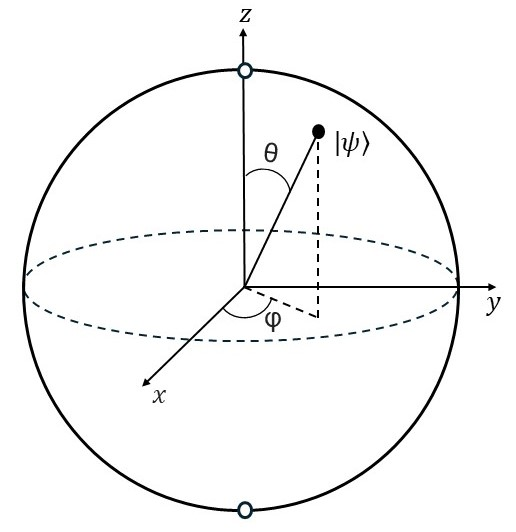
\includegraphics[width=0.35\textwidth]{images/bloch_sphere.jpg}
  \caption{Bloch sphere representation of a qubit}
  \label{fig:bloch_sphere}
\end{figure}

The distance between two quantum states $\ket{\psi}$ and $\ket{\psi'}$ is their Euclidean distance in the Bloch sphere \cite{wallman2016noise,nielsen2010quantum}. 

There are infinite points in the Bloch sphere, which might suggest the possibility of encoding an infinite amount of information in the infinite binary expansion of the angle $\theta$. However, when a qubit is measured, it collapses to one of the basis states, so only one bit of information can be extracted from a qubit. To accurately determine the amplitudes $\alpha$ and $\beta$, an infinite number of identical qubit copies would need to be measured. Nevertheless, it is still conceptually valid to think of these amplitudes as ``hidden information''. One could say that quantum computation is the art of manipulating this hidden information using phenomena such as interference and superposition to perform tasks that would be impossible or inefficient with classical computers.


% Nota sobre parte final do chuang: informação codificada num qubit e o que perdemos qd medimos um qubit
% Computação quantica é a arte de manipular a informação escondida nos estados quanticos (fenomenos como interferencia e superposição) para realizar tarefas que seriam impossiveis ou ineficientes com computadores clássicos.

\subsection{Multi-qubit States} \label{subsec:entanglement}

\begin{definition}
 The state space of a composite physical system is the tensor product of the state spaces of the component physical systems. As a result, an $n$\emph{-qubit state} can be represented by a unit vector in $2^n$-dimensional Hilbert space, $\mathbb{C}^{2^{n}}$. The notations \gls{states-otimes}, \gls{states-no-otimes}, and \gls{states-2gether} are  used to denote the tensor product of two states $\ket{\psi}$ and $\ket{\phi}$. As for any complex vector, $\ket{\psi}^{\otimes n}$ denotes the n-fold tensor product of state $\ket{\psi}$ with itself. The computational basis states of an $n$-qubit system are of the form $\ket{x_{1}\ldots x_{n}}$ and so a quantum state of such a system is specified by $2^{n}$ amplitudes. For instance, a two-qubit state can be written as
\begin{equation*}
  \ket{\psi} = \alpha_{00}\ket{00} + \alpha_{01}\ket{01} + \alpha_{10}\ket{10} + \alpha_{11}\ket{11}.
\end{equation*}
\end{definition}
It should be noted that unfortunately, no simple generalization of the Bloch sphere known for multiple qubits.

%falta n-fold
%ir ao tensor e acrecentar os operadores que mapeiam operadores

\subsubsection{Entanglement}

\begin{definition}
  An interesting aspect of multi-qubit states is the phenomenon of \emph{entanglement}. This term means strong intrinsic correlations between two (or more) particles when the quantum state of each of them cannot be described independently of the state of the other, \text{i.e.} cannot be written as a product of states of the individual qubits. Measuring one qubit of the entangled pair affects the state of the other qubit. This must happen even if the particles are far apart.
\end{definition}

In order to better understand this concept, consider the follow \emph{Bell state} or \emph{EPR pair}:
\begin{equation*}
  \ket{\Phi^{+}} = \frac{1}{\sqrt{2}}(\ket{00} + \ket{11}).
\end{equation*}

Upon measuring the first qubit, there are two possible outcomes: $0$ with probability $1/2$ and $1$ with probability $1/2$. If the first qubit is measured to be $0$, the second qubit will also be $0$ with probability 1. If the first qubit is measured to be $1$, the second qubit will also be $1$ with probability 1. Therefore, the measurement outcomes are correlated.

These correlations prompted Einstein, Podolsky, and Rosen to publish a paper \cite{einstein1935can} questioning the completeness of quantum mechanics in 1935. The EPR paradox presented a dilemma: the existence of entanglement (\text{i.e.}, correlations that persist regardless of distance) versus local realism and hidden variables. Einstein argued that if two objects, which have interacted in the past but are now separated, exhibit perfect correlation, they must possess a set of properties determined before their separation. These properties would persist in each object, dictating the outcomes of measurements on both sides. Einstein believed that the strong correlations predicted by quantum mechanics necessitate the existence of additional properties not accounted for by the quantum formalism that determine the measurement results. Therefore, he argued that quantum mechanics might require supplementation, as it may not represent a complete or ultimate description of reality.


In 1964, John Bell made a remarkable discovery: the measurement correlations in the Bell state are stronger than those that could ever occur between  classical systems \cite{bell1964einstein}. He explored the idea that each entangled particle might possess hidden properties — unaccounted for by quantum mechanics—that determine the measurement outcomes. Then, through mathematical reasoning, Bell demonstrated that the correlations predicted by any local hidden variable theory cannot exceed a specific level.  There is an upper limit of correlations fixed by what today is called the ``Bell inequalities". He found that quantum theory sometimes predicts correlations that exceed this limit. Consequently, an experiment could  settle the debate by testing whether or not correlations surpass the bounds he had found following Einstein's position.


In 1982, Alain Aspect conducted an experiment that confirmed the violation of the Bell inequalities \cite{aspect1982experimental}. In this experiment, polarizers were placed more than twelve meters apart. This meant that the correlation obtained could not be explained by the fact that the particles carry within them unmeasured properties. Moreover, it proved that the outcome of the measurement is not determined until the moment of measurement. There seemed to be an instantaneous exchange between two particles at the time of measurement when they were twelve meters apart.



Sixteen years later, Nicolas Gisin \cite{tittel1998experimental} and Anton Zeilinger \cite{pan1998experimental} conducted similar experiments, demonstrating that entanglement persists over distances of several kilometers. More recently,  \cite{yin2017satellite} extended these tests using entangled photon pairs sent from a satellite to verify Bell's inequalities over a distance of one thousand kilometers, further confirming that, regardless of the distance, entangled particles behave as an indivisible, inseparable whole. The connection between them is so profound that it appears to challenge the principles of relativity. This phenomenon is known as \emph{quantum nonlocality}.

\subsection{Unitary operators and Measurements}\label{subsec:unitary-operators&measurements}




\subsubsection{Pauli Matrices}
\begin{definition}
The Pauli matrices are a set of three $2 \times 2$ hermitian matrices that are defined as follows:
\begin{equation*}
  \sigma_{x} = \begin{pmatrix} 0 & 1\\ 1 & 0 \end{pmatrix}, \hspace{1cm} \sigma_{y} = \begin{pmatrix} 0 & -i\\ i & 0 \end{pmatrix}, \hspace{1cm} \sigma_{z} = \begin{pmatrix} 1 & 0\\ 0 & -1 \end{pmatrix}.
\end{equation*}
\end{definition}

The eigenvectors and eigenvalues of the Pauli matrices are as follows:
\begin{align*}
 & \sigma_{x} \begin{pmatrix} 1 \\ 1 \end{pmatrix} = \begin{pmatrix} 1 \\ 1 \end{pmatrix}, \hspace{1.4cm} \sigma_{y} \begin{pmatrix} 1 \\ i \end{pmatrix} =  \begin{pmatrix} 1 \\ i \end{pmatrix}, \hspace{1.4cm} \sigma_{z} \begin{pmatrix} 1 \\ 0 \end{pmatrix} = \begin{pmatrix} 1 \\ 0 \end{pmatrix} \\
  & \sigma_{x} \begin{pmatrix} 1 \\ -1 \end{pmatrix} = -\begin{pmatrix} 1 \\ -1 \end{pmatrix}, \hspace{0.7cm} \sigma_{y} \begin{pmatrix} 1 \\ -i \end{pmatrix} = -\begin{pmatrix} 1 \\ -i \end{pmatrix}, \hspace{0.7cm} \sigma_{z} \begin{pmatrix} 0 \\ 1 \end{pmatrix} = -\begin{pmatrix} 0 \\ 1 \end{pmatrix}.
\end{align*}

The normalized eigenvectors of $\sigma_x$ are $\ket{+} = \frac{1}{\sqrt{2}}(\ket{0} + \ket{1})$ and $\ket{-} = \frac{1}{\sqrt{2}}(\ket{0} - \ket{1})$, and normalized eigenvectors of $\sigma_y$ are $\ket{+i} = \frac{1}{\sqrt{2}}(\ket{0} + i\ket{1})$ and $\ket{-i} = \frac{1}{\sqrt{2}}(\ket{0} - i\ket{1})$. The eigenvectors of $\sigma_z$ are $\ket{0}$ and $\ket{1}$. These eigenvectors correspond to the $\hat{x}, \hat{y}$ and $\hat{z}$ axes of the Bloch sphere in \autoref{fig:bloch_sphere}, respectively.

When matrices $\sigma_x, \sigma_y$ or  $\sigma_z$ are applied to a state on the Bloch sphere, they rotate the state by $\pi$ radians around the $\hat{x}, \hat{y}$ or $\hat{z}$ axis, respectively. For example, the action of $\sigma_x$ on the state $\ket{0}$ is to rotate it to $\ket{1}$, and vice versa. Note that for the eigenstates of these matrices with eigenvalue $-1$, this still applies if considering a global phase of $-1 = e^{i\pi}$, given that two quantum states $\ket{\psi}$ and $e^{i\phi}\ket{\psi}$ are indistinguishable by any quantum measurement.

Matrices $\sigma_x$ and $\sigma_z$ will also be referred to as \gls{x} and \gls{z}, respectively.

\subsubsection{Unitary operators}
\begin{definition}
  \emph{Closed systems}, \text{i.e.}, systems that do not interact with other systems evolve according to unitary operators. In quantum computation, these unitary operators are also known as \emph{gates}. For a  state $\ket{\psi}$, a \emph{unitary operator} $U$ describes an evolution from $\ket{\psi}$ to $ U\ket{\psi}$.
\end{definition}

\begin{example}
Pauli matrices are examples of unitary operators. The $X$ and $Z$ gates are often referred to as the \emph{not} and \emph{phase flip} gates, respectively. Other important unitary operators include   \emph{Hadamard gate}, denoted \gls{h}, which maps $\ket{0}$ to $\ket{+}$ and $\ket{1}$ to  $\ket{-}$, and the \emph{phase-shift gate}, denoted \gls{p}, which leaves $\ket{0}$ unaltered applies a phase shift of $\theta$ to the state $\ket{1}$:
\begin{equation*}
 H = \frac{1}{\sqrt{2}}\begin{pmatrix} 1 & 1\\ 1 & -1 \end{pmatrix}, \hspace{1cm} P = \begin{pmatrix} 1 & 0\\ 0 & e^{i \theta} \end{pmatrix}.
\end{equation*}
 
When the Pauli matrices are exponentiated, they result in three valuable classes of unitary matrices, corresponding to the rotation operators around the $\hat{x}$, $\hat{y}$, and $\hat{z}$ axes, which are defined as follows:
\begin{equation*}
  R_{x}(\theta) = e^{-i\theta \sigma_{x}/2} = \text{cos} \left(\frac{\theta}{2} \right) \id -i \text{sin} \left(\frac{\theta}{2} \right) \sigma_{x} = \begin{pmatrix} \cos(\frac{\theta}{2}) & -i\sin(\frac{\theta}{2})\\ -i\sin(\frac{\theta}{2}) & \cos(\frac{\theta}{2}) \end{pmatrix},
\end{equation*}
\begin{equation*}
  R_{y}(\theta) = e^{-i\theta \sigma_{y}/2} = \text{cos} \left(\frac{\theta}{2} \right) \id -i \text{sin} \left(\frac{\theta}{2} \right) \sigma_{y} = \begin{pmatrix} \cos(\frac{\theta}{2}) & -\sin(\frac{\theta}{2})\\ \sin(\frac{\theta}{2}) & \cos(\frac{\theta}{2}) \end{pmatrix},
\end{equation*}
\begin{equation*}
  R_{z}(\theta) = e^{-i\theta \sigma_{z}/2} = \text{cos} \left(\frac{\theta}{2} \right) \id -i \text{sin} \left(\frac{\theta}{2} \right) \sigma_{z} = \begin{pmatrix} e^{-i\theta/2} & 0\\ 0 & e^{i\theta/2} \end{pmatrix}.
\end{equation*}
\end{example}

\begin{theorem} \label{unitary} \cite{nielsen2010quantum}
  Suppose $U$ is a unitary operation on a single qubit. Then there exist real numbers $\alpha$, $\beta$, $\gamma$ and $\delta$ such that
  \begin{equation*}
    U = e^{i\alpha} R_{z}(\beta) R_{y}(\gamma) R_{z}(\delta).
  \end{equation*}
\end{theorem}

\begin{example}
  
There are also multi-qubit gates, such as the \emph{controlled-not} gate, denoted \gls{cnot}, which leaves the states $\ket{00}$ and  $\ket{01}$ unchanged, and maps $\ket{10}$ and $\ket{11}$ to each other:
\begin{equation*}
  \textit{CNOT} = \begin{pmatrix} 1 & 0 & 0 & 0\\ 0 & 1 & 0 & 0\\ 0 & 0 & 0 & 1\\ 0 & 0 & 1 & 0 \end{pmatrix}.
\end{equation*}
In this case, as the state of the first qubit determines if the $X$ gate is applied to the second qubit, the first qubit is called the \emph{control qubit} and the second qubit the \emph{target qubit}. 

There is an ``extension" of the controlled-not gate, the controlled-$U$ gate, where $U$ is a unitary gate acting on a single qubit. This gate applies the gate $U$ to the target qubit if the control qubit is in state $\ket{1}$ and does nothing otherwise. It is defined as:
\begin{align*}
  &\textit{CU} (\ket{0} \otimes \ket{\psi}) = \ket{0} \otimes \ket{\psi}\\ 
  &\textit{CU} (\ket{1} \otimes \ket{\psi}) = \ket{1} \otimes U\ket{\psi}.
\end{align*}
\end{example}

It should be noted that no completely closed systems exist in the universe. Nevertheless, for many systems, the approximation of a closed system is valid.
% No fim nota sobre não haver sistemas completamente fechados no universo, mas que a aproximação de um sistema fechado é válida para muitos sistemas, p.82



\subsubsection{Measurements}

% decidir se e como por M0 e M1

There are times when it necessary to observe the system to extract information. This interection leaves the system no longer closed and, consequently, the evolution of the system is no longer unitary. 

\begin{definition}
The act of measuring a qubit is represented by a set of operators called \emph{measurement operators}, denoted $\{M_{m}\}$. These operators act on the state space  of the system being measured. The index $m$ refers possible measurement outcomes. These measurement operators must satisfy the completeness equation $\sum_{m} M_{m}^{\dagger}M_{m} = \id$, which ensures that the probabilities of all possible outcomes sum to 1. If a measurement ${M_m}$ is performed on a state $\ket{\psi}$ the outcome $m$ is observed with probability $p_m = \bra{\psi}M_{m}^{\dagger}M_{m}\ket{\psi}$ for each $m$. Moreover, after a measurement yielding outcome $m$, the state collapses to 
\begin{align*}
  \ket{\psi'}=\frac{M_{m}\ket{\psi}}{\sqrt{p_{m}}}.
\end{align*}
\end{definition}

\begin{example}
In the case of the computational basis, the measurement operators are the projectors onto the basis states $\ket{0}$ and $\ket{1}$ denoted by $M_{0} = \ket{0}\bra{0}$ and $M_{1} = \ket{1}\bra{1}$, respectively. Considering an arbitrary state $\ket{\psi} = \alpha \ket{0} + \beta \ket{1}$, the probabilities of measuring 0 and 1 are $p_0 = \bra{\psi} M_{0} M_{0}^{\dag}\ket{\psi}=\bra{\psi} M_{0} \ket{\psi} = |\alpha|^{2}$, and $p_1 = \bra{\psi} M_{1} M_{1}^{\dag}\ket{\psi} = \bra{\psi} M_{1} \ket{\psi} =  |\beta|^{2} $, respectively. Consequently the states after measurement are
\begin{align*}
  &\ket{\psi'}=\frac{M_{0}\ket{\psi}} {|\alpha|} = \frac{\alpha}{|\alpha|} \ket{0} = \ket{0} (\text{with  } p=p_0) \quad \text{and } \\
  &\ket{\psi''}= \frac{M_{1}\ket{\psi}} {|\beta|} = \frac{\beta}{|\beta|} \ket{1} = \ket{1} (\text{with  } p=p_1)
\end{align*}
\end{example}


From now on, unless stated otherwise, any reference to measurement should be understood as pertaining to the computational basis.

As previously mentioned, any states $\ket{\psi}$ and $e^{i\phi}\ket{\psi}$ are indistinguishable by any quantum measurement. Consider a measurement operator $M_m$, the probabilities of obtaining outcome $m$ are $\bra{\psi} M_{m}^{\dagger}M_{m}\ket{\psi}$ and $\bra{\psi} e^{-i \theta} M_{m}^{\dagger}M_{m}e^{i\theta}\ket{\psi}=\bra{\psi} M_{m}^{\dagger}M_{m}\ket{\psi}$. For this reason, it is said that these states are equal from an observational point of view.



%If a measurement ${M_m}$ is performed on a state $\rho$, the outcome $m$ is observed with probability $p_m = \text{Tr}(M_{m} \rho M^{\dag}_{m})$ for each $m$. Moreover, after a measurement yielding outcome $m$, the state collapses to $M_{m}\rho M^{\dag}_{m}/p_{m}$. 
% ver p.93

\subsection{Density operators}
Until now the state vector formalism was used. However there is an alternative formulation using density operators. The density operator is often known as the \emph{density matrix}, the two terms will be used interchangeably.

%\subsubsection{General properties}

\begin{definition}
A quantum state $\ket{\psi}$ is said to be a \emph{pure state} if it is completely known, \ie if it can be written as a ket. In this case, the state can be written in the density operator formalism as $\rho = \ket{\psi}\bra{\psi}$. 
\end{definition}

\begin{definition}
A state that is a probabilistic mixture of pure states is designated a \emph{mixed state}. A mixed state $\sum_i \alpha_i \ket{\psi_i}$ can be represented by a density operator $\rho= \sum_i |\alpha_i|^{2}\ket{\psi_i}\bra{\psi_i}$. Note that $|\alpha_i|^{2}$ is the probability of the system being in state $\ket{\psi_i}$.
\end{definition} 

\begin{definition}[Unitary Evolution of a Density Operator]
  When a unitary operator \( U \) is applied to a quantum state described by a density matrix \( \rho \), the resulting state is given by $ \rho' = U \rho U^\dagger.$
\end{definition}

\begin{definition}[Measurement of a Density Operator]
  Given a collection of measurement operators \( \{M_m\} \), the probability of obtaining outcome \( m \) when measuring a state \( \rho \) is $p_m = \text{Tr}(M_m \rho M_m^\dagger).$
  After observing outcome $ m $, the post-measurement state collapses to:
  \[
  \rho' = \frac{M_m \rho M_m^\dagger}{\text{Tr}(M_m \rho M_m^\dagger)}.
  \]
\end{definition}


\begin{definition}
  In \autoref{subsec:hilb2D} it was shown how to determine the cartesian coordenates of a pure state in the Bloch sphere from the state vector. For an arbitrary $2 \times 2$ density matrix, the following holds
\begin{equation} \label{eq:bloch_vector_0}
  \rho = \frac{1}{2}(\id + r_{x}\sigma_{x} + r_{y}\sigma_{y} + r_{z}\sigma_{z}),
\end{equation}
where $r = (r_x, r_y, r_z)$ is a real three-dimensional vector such that $\| r \|_2 \leq 1$. This vector is known as the \emph{Bloch vector for the state} $\rho$. Since $\rho$ is Hermitian. $r_x, r_y$ and $r_z$ are always real.  The inverse map of \autoref{eq:bloch_vector_0} is
\begin{equation}
  \label{eq:Bloch_vector}
  r_{\mu} = \text{Tr}(\rho \sigma_{\mu})
  \end{equation} 
\end{definition}


  Note that given that the trace is linear and matrix multiplication distributes over matrix addition, the cartesian coordinates of an operator consisting of the sum or subtraction of density operators can also be determined by \autoref{eq:Bloch_vector}.

\subsubsection{Reduced density operator}

Density operators are particularly well-suited for describing individual subsystems of a composite quantum system. This type of description is provided by the \emph{reduced density operator}

\begin{definition}
Let \( \ket{a_1}, \ket{a_2} \) be vectors in the Hilbert space of system \( A \), and \( \ket{b_1}, \ket{b_2} \) vectors in the Hilbert space of system \( B \). The \emph{partial trace over} \( B \) is defined by:
\begin{align*}
  \text{Tr}_{B}(\ket{a_1}\bra{a_2} \otimes \ket{b_1}\bra{b_2}) & =\ket{a_1}\bra{a_2}\text{Tr}(\ket{b_1}\bra{b_2}) \\
  & = \ket{a_1}\bra{a_2}  \sum_{\mu} \bra{\mu} \ket{b_1}\bra{b_2} \ket{\mu} \\
  & =  \ket{a_1} \bra{a_2} \sum_{\mu} \braket{\mu} {b_1}\braket{b_2} {\mu} \\
  & = \ket{a_1} \bra{a_2} \sum_{\mu} \braket{b_2}{\mu} \braket{\mu}{b_1} \\
  &= \ket{a_1}\bra{a_2}  \braket{b_2}{b_1}
\end{align*}
where \( \{\ket{\mu}\} \) is an orthonormal basis spanning the state space of \( B \).
In certain situations it is more advantageous to consider the reduced density operator for subsystem $A$ defined as:
\begin{equation*}
  \rho_{A} = \text{Tr}_{B}(\rho_{AB}) = \sum_{\mu} \bra{\mu} \rho_{AB} \ket{\mu},
\end{equation*}
where $\{\ket{\mu}\}$, span the state space of $B$ and act only in the state space of $B$. 
\end{definition}

\begin{definition}
Given physical systems $A$ and $B$ whose composite system is given by the density operator $\rho_{AB}$, the \emph{reduced density operator} for subsystem $A$ is $$\rho_{A} = \text{Tr}_{B}(\rho_{AB}).$$ 

Note that, by linearly, the partial trace of $\rho_{AB} = \sum_{ijkl} p_{ijkl} \ket{a_i} \bra{a_j}  \otimes \ket{b_k} \bra{b_l}$ is
\begin{align*}
  \text{Tr}_{B}(\rho_{AB}) &= \sum_{ijkl} p_{ijkl} \text{Tr}_{B}\left(\ket{a_i}\bra{a_j} \otimes \ket{b_k} \bra{b_l}\right) \\
  & = \sum_{ijkl} p_{ijkl} \ket{a_i}\bra{a_j}  \sum_{\mu} \braket{b_l}{\mu} \braket{\mu}{b_k}= \sum_{ijkl} p_{ijkl} \ket{a_i}\bra{a_j}   \braket{b_l}{b_k} 
\end{align*} 

Similarly, the \emph{reduced density operator for subsystem} $B$ is $\rho_{B} = \text{Tr}_{A}(\rho_{AB})$.
\end{definition}




 %\begin{align*}
 %\text{Tr}_{B}(\ket{a}\bra{b} \otimes \ket{c}\bra{d}) & =\ket{i}\bra{j} \text{Tr}(\ket{k}\bra{l}) \\
 %&= \ket{a}\bra{b} \sum_{\mu} \bra{\mu} \ket{c}\bra{d}  \ket{\mu} \\
 %& = \sum_{\mu} \bra{\mu} \ket{a} \bra{b} \otimes \ket{c} \bra{d} \ket{\mu} 
%\end{align*}
%where $\ket{a}$ and $\ket{b}$ are any two vectors in the state space of $A$,  $\ket{c}$ and $\ket{d}$ are any two vectors in the state space of $B$, and $\{\ket{\mu}\}$, span the state space of $B$, act only in the state space of $B$. Therefore, by linearly, the partial trace of $\rho_{AB} = \sum_{ij} p_{ij} \ket{a_i} \bra{b_i}  \otimes \ket{c_j} \bra{d_j}  $ is




%An $n$-qubit mixed state can be represented by a density operator $ \mathbb{C}^{2^{n}} \xrightarrow{} \mathbb{C}^{2^{n}}$, whose matrix representation is $\rho = \Sigma_{i} \hspace{2pt} p_{i} \vert \phi_{i} \rangle \langle \phi_{i} \vert$. A density operator encodes uncertainty about the current state of the quantum system at hand. For example, a mixed state with half probability of $\vert 0 \rangle$ and $\vert 1 \rangle$ can be represented by $\frac{\vert 0 \rangle \langle 0 \vert + \vert 1 \rangle \langle 1 \vert}{2}=I/2$, where $I$ is the identity matrix.  One usually denotes density matrices by the greek letters $\rho$, $\sigma$, and so forth. The set of density operators is denoted by $\mathcal{D}_{n} \subseteq \mathbb{C}^{ 2^{n \times n}}$.

% tudo sobre matrizes de densidade incuindo a definição de matriz de densidade reduzida e traço parcial

% bloch vector for mixed states

\todo[inline,size=\normalsize]{Decidir onde colocar a def de trace-nonincreasing op e quantum operation: aqui ou na parte das contribuições qd falar da categoria do selinger} 

\subsection{Quantum Channels} \label{subsec:quantum_channels}

% Fazer secção chamada quantum chanels e falar de super operadores e cptp maps, normas, kraus operators

Thus far, only two types of quantum operations have been discussed: unitary operators, which describe the evolution of a closed quantum system, and measurements, which describe the act of observing a quantum system. Now, a new type of quantum operation that accounts for the more realistic notion of interaction between a quantum system and an environment will be introduced. Nonetheless, it is necessary to first introduce a few key concepts.



%the evolution of a quantum system has been described by unitary operators. However, in practice, quantum systems are not isolated, and they interact with their environment. This interaction is described by a \emph{quantum channel}, which is a completely positive trace-preserving (CPTP) linear map. A quantum channel is a generalization of a unitary operator that allows for the description of the evolution of a quantum system under the influence of an environment.

\begin{definition}
  A \emph{super-operator} $Q$ is a linear map between the space of operators on a Hilbert space. 
\end{definition}

\begin{definition} \label{def:positive_superoperator}
  A super-operator $Q$ is called \emph{positive} if it sends positive matrices to positive matrices, \textit{i.e.} $A \geq 0 \Rightarrow{} Q A \geq 0$.
\end{definition}

\begin{definition} \label{def:completely_positive_superoperator}
  A super-operator $Q$ is said to be \emph{completely positive} if for all $k$, 
  $$Q \otimes I_{\mathbb{C}^{k \times k}}: \mathbb{C}^{n \times n} \otimes \mathbb{C}^{k \times k} \rightarrow \mathbb{C}^{m \times m} \otimes \mathbb{C}^{k \times k}  $$
   is positive.
  %A super-operator $Q : V \rightarrow W$ is said to be \emph{completely positive} if for all $R$, $Q \otimes I_{R}: V \otimes R \rightarrow W \otimes R$
   %is positive.
\end{definition}

\begin{definition} \label{def:trace_preserving_superoperator}
  A super-operator $Q$ is called \emph{trace-preserving} if $\text{Tr} \hspace{2pt} (Q A)= \text{Tr} (A)$.
\end{definition}

Since density matrices are positive, any physically allowed transformation must be represented by a positive operator. Nonetheless, this is not sufficient on its own: since one can always extend the space $\mathbb{C}^{n \times n}$ to  $\mathbb{C}^{n \times n} \otimes \mathbb{C}^{m \times m} $ by adjoining a new quantum system, any physically allowed transformation must be completely positive. Finally, since the trace of a density matrix is always $1$, any physically allowed transformation must be trace-preserving. 

\begin{definition}
  A \acrfull{cptp} operator is traditionally called a \emph{quantum channel}.
\end{definition}



\subsubsection{Kraus operator sum representation}


Assume that there is a quantum system $S$ of interest which is a subsystem of a larger system which also includes an environment $E$. These systems have a joint unitary evolution described by a unitary operator $U$ acting on the composite system, $U (\rho_{SE} )= U \rho_{SE} U^{\dag}$. 

Given that density matrices are positve operators, by (\autoref{def:positive}), the density operator of the environment $\rho_E$ initially can be written as 
\begin{equation*}
  \rho_E = \sum_{i} p_{i} \ket{i} \bra{i}
\end{equation*}
where $\ket{i}$ form an orthonormal basis for the state space of $E$ and $p_{i}$ are positive. 

The state of the subsystem $S$ after the unitary evolution corresponds to the partial trace of the joint state over the environment,
\begin{align*}
  \rho_{S}' = & \text{Tr}_{E}(U \rho_{SE} U^{\dag}) \\
 = & \sum_{\mu} \bra{\mu} U \rho_{SE} U^{\dag} \ket{\mu}
\end{align*}
where $\{\ket{\mu}\}$ span the state space of $E$.

 
Considering that initially both systems are completely decoupled, the initial state of the system can be written as $ \rho_{SE} = \rho_{S} \otimes \rho_{E}$. Thus,
\begin{align*} 
  \rho_{S}' = & \sum_{\mu} \bra{\mu} U \rho_{S} \otimes \sum_{i} p_{i} \ket{i} \bra{i} U^{\dag} \ket{\mu} \\
  = & \sum_{\mu i}  \sqrt{p_{i}} \bra{\mu} U \ket{i} \rho_{S} \sqrt{p_{i}} \bra{i} U^{\dag} \ket{\mu}  \\ 
  = & \sum_{\mu i} \text{K}_{\mu i} \rho_{S} \text{K}_{\mu i}^{\dag}
\end{align*}
where the set of operators $\{\text{K}_{\mu i}\}$ is designated \emph{Kraus operators} and $\text{K}_{\mu i} = \sqrt{p_{i}} \bra{\mu} U \ket{i}$. Note that $\{\ket{\mu}\}$ and $\{\ket{i}\}$, act only in the state space of $E$. 

\begin{definition}
  The equation $ \rho_{S}' = \sum_{\mu i} \text{K}_{\mu i} \rho_{S} \text{K}_{\mu i}^{\dag} $ is called an \emph{\acrfull{osr}}. An \acrshort{osr} can be thought of as a quantum channel that maps $\rho_{S}$ to $\sum_{\mu i} \text{K}_{\mu i} \rho_{S} \text{K}_{\mu i}^{\dag}$, given this map is \acrshort{cptp} \cite{lidar2019lecture, watrous2018theory}. 
\end{definition}




\subsubsection{Non-selective measurements}

In the previously presented formalism to represent all the possible outcomes of a measurement, described by a set of operators $\{M_{m}\}$, on a state $\rho$, it would be necessary to write that state $\rho$ collapse to state $\rho_m=\frac{M_{m}^{\dag}\rho M_{m}}{\text{Tr}(M_{m}\rho M_{m}^{\dag})}$ with probability $p_m=\text{Tr}(M_{m}\rho M_{m}^{\dag})$, for each possible outcome $m$. Although the selective description above is useful conceptually, it is often impractical for calculations. Instead, one uses \emph{non-selective measurements}, in which the possible outcomes are not explicitly stated.


\begin{definition}
A \emph{non-selective measurement} is a quantum measurement in which the post-measurement state of the system is then given by the weighted sum over all possible outcomes:
\[
\rho = \sum_m p(m) \rho_m = \sum_m M_m \rho M_m^{\dag}.
\]
This last equality corresponds to an Kraus operator sum representation, where the set of Kraus operators is $\{M_{m}\}$.
\end{definition}



\subsubsection{Norms on quantum channels}
\begin{definition} \label{def:trace_norm_superoperator}
  The norm of a super-operator $Q: \mathbb{C}^{n\times n} \xrightarrow{} \mathbb{C}^{m\times m }$ is defined:
  \begin{equation*} 
    \lVert Q \rVert_{1} =  \max\{\lVert Q \hspace{1pt} A \rVert_{1}   \mid  \lVert A \rVert_{1}=1\}, 
  \end{equation*}
\end{definition}
where $A \in \mathbb{C}^{n \times n }$

%\begin{theorem} \label{thm:Russo–Dye} \cite[Theorem 3.39]{watrous2018theory}
  %Let $Q: \mathbb{C}^{n \times n} \rightarrow \mathbb{C}^{m \times m}$ be a positive super-operator and $u \in \mathbb{C}^{n}$. It holds that 
  %\begin{equation}
    %\lVert Q \rVert_{1} = \max \{\text{Tr}\left(Q(uu^{*}) \right) \vert \hspace{2pt}  \lVert u \rVert_{1}=1 \}.
  %\end{equation}
%\end{theorem}

%\begin{proposition} \cite[Proposition 3.41]{watrous2018theory}
%The following facts hold for the trace norm:
%\begin{enumerate}
  %\item The trace norm is submultiplicative with respect to composition of super-operators , \textit{i.e.}, for all super-operators  $Q: \mathbb{C}^{n \times n} \rightarrow \mathbb{C}^{m \times m}$ and $S: \mathbb{C}^{m \times m} \rightarrow \mathbb{C}^{o \times o}$
  %\begin{equation}
    %\lVert S  Q \rVert_{1} \leq \lVert S \rVert_{1} \lVert Q \rVert_{1}.
  %\end{equation}
  %\item Let $U_0,$ $V_0 \in \mathbb{C}^{n\times n}$ and $U_1,$ $V_1 \in \mathbb{C}^{m\times m}$ be unitary operators, let $Q,$ $S: \mathbb{C}^{n \times n} \rightarrow \mathbb{C}^{m \times m}$ be super-operators, where $S$ is defined as:
  %\begin{equation}
    %S(X) = U_1 Q(U_0 A V_0) V_1
 % \end{equation}
  %for all $A \in \mathbb{C}^{n\times n}$. It holds that $\lVert Q \rVert_{1} = \lVert S \rVert_{1} $.
%\end{enumerate}
%\end{proposition}


Unfortunately, this norm is not stable under tensoring , given that the inequation $ \lVert Q \otimes I_{\mathbb{C}^{n\times n}} \rVert_{1} \leq \lVert Q \rVert_{1}$ does not hold \cite{watrous2018theory}. As a result, the diamond norm, which is based on the trace norm, is used instead in the context of quantum channels. 

\begin{definition}
  Given a super-operator $Q: \mathbb{C}^{n\times n} \xrightarrow{} \mathbb{C}^{m\times m }$, the diamond norm, \gls{diamond-norm} , is defined as:
  \begin{equation*}  \label{eq:diamond_distance}
    \lVert Q \rVert_{\diamondsuit} =  \lVert Q \otimes \id_{\mathbb{C}^{n \times n}} \rVert_{1}
  \end{equation*}
\end{definition}
%where $I_{\mathbb{C}^{n \times n}} $ is the identity super-operator over the space $\mathbb{C}^{n\times n}$.

%3.46
%For all super-operators $Q: \mathbb{C}^{n \times n}\rightarrow \mathbb{C}^{m \times m} $, it holds that 
%\begin{equation}
  %\lVert Q \rVert_{\diamondsuit} \geq \lVert Q \otimes I_{\mathbb{C}^{o\times o}} \rVert_{1},
%\end{equation}
%if $\text{dim}(\mathbb{C}^{o\times o}) \geq \text{dim}(\mathbb{C}^{n\times n})$.

For this norm it holds that for all super-operators $Q: \mathbb{C}^{n \times n}\rightarrow \mathbb{C}^{m \times m} $ and $S:\mathbb{C}^{m \times m} \rightarrow \mathbb{C}^{o \times o} $, if $Q$ is a quantum channel then $\lVert S  Q \rVert_{\diamondsuit} \leq \lVert S \rVert_{\diamondsuit}$ \cite[Proposition 3.44 and Proposition 3.48]{watrous2018theory}, and if $S$ is a quantum channel, then $\lVert S  Q \rVert_{\diamondsuit} \leq \lVert Q \rVert_{\diamondsuit}$. This is a desireble property, as is guarantees that quantum operations do not increase the distance between states, and as a
consequence, composition of programs is valid.
%Moreover, the following inequalties hold for a super-operator $Q$: $ \lVert Q \rVert_{\diamondsuit} \geq \lVert Q \otimes I \rVert_{\diamondsuit} $ and $\lVert Q \rVert_{\diamondsuit} \geq \lVert I \otimes Q  \rVert_{\diamondsuit} $
%3.44
%\begin{proposition} \cite[Proposition 3.44]{watrous2018theory}
   %For all quantum channels $Q:\mathbb{C}^{n \times n}\rightarrow \mathbb{C}^{m \times m}$, it holds that $\lVert Q \rVert_{\diamondsuit} = 1$.
%\end{proposition}

%\begin{theorem} \label{thm:tensor_stability} \cite[Theorem 3.46 ]{watrous2018theory}
%For all super-operators $Q:\mathbb{C}^{n \times n}\rightarrow \mathbb{C}^{m \times m}$ and complex spaces $\mathbb{C}^{o\times o}$  it holds that:
%\begin{equation}
  %\lVert Q \otimes I_{\mathbb{C}^{o\times o}} \rVert_{1} \leq  \lVert Q \rVert_{\diamondsuit}. 
%\end{equation}
%with equality holding under the assumption that $\text{dim}(\mathbb{C}^{o\times o}) \geq  \text{dim}(\mathbb{C}^{n \times n})$.
%\end{theorem}

%\begin{corollary} \label{cor:diamond_otimes_I} \cite[Corollary 3.47]{watrous2018theory}
   %For all super-operators $Q:\mathbb{C}^{n \times n}\rightarrow \mathbb{C}^{m \times m}$ and complex spaces $\mathbb{C}^{o\times o}$  it holds that:
  %\begin{equation}
    %\lVert Q \rVert_{\diamondsuit} = \lVert Q \otimes I_{\mathbb{C}^{o\times o}} \rVert_{\diamondsuit} .
  %\end{equation}
%\end{corollary}

%\begin{proposition} \cite[Proposition 3.48]{watrous2018theory}
  %Moreover the following properties hold for the diamond norm:
  %\begin{enumerate}
    %\item The diamond norm is submultiplicative with respect to composition of , \textit{i.e.}, for all super-operators $Q: \mathbb{C}^{n \times n} \rightarrow \mathbb{C}^{m \times m}$ and $S: \mathbb{C}^{m \times m} \rightarrow \mathbb{C}^{o \times o}$, it holds that:
  %\begin{equation}
    %\lVert S  Q \rVert_{\diamondsuit} \leq \lVert S \rVert_{\diamondsuit} \lVert Q \rVert_{\diamondsuit}.
  %\end{equation}
  %\item For all super-operators $Q_0, S_0: \mathbb{C}^{n \times n} \rightarrow \mathbb{C}^{m \times m}$ and $Q_1, S_1: \mathbb{C}^{m \times m} \rightarrow \mathbb{C}^{o \times o}$, it holds that:
  %\begin{equation}
  %\lVert S_1 S_0 - Q_1 Q_0  \rVert_{\diamondsuit} \leq \lVert S_0 - Q_0 \rVert_{\diamondsuit} + \lVert S_1 - Q_1 \rVert_{\diamondsuit}.
  %\end{equation}
%\end{enumerate}
%\end{proposition}

%\begin{theorem} \cite[Theorem 3.49]{watrous2018theory}
  %\item The diamond norm is multiplicative with respect to tensor products, \textit{i.e.}, for all super-operators $Q: \mathbb{C}^{n \times n} \rightarrow \mathbb{C}^{m \times m}$ and $S: \mathbb{C}^{o \times o} \rightarrow \mathbb{C}^{p \times p}$, it holds that:
  %\begin{equation}
    %\lVert Q \otimes S \rVert_{\diamondsuit} = \lVert Q \rVert_{\diamondsuit} \lVert S \rVert_{\diamondsuit}.
  %\end{equation}
%\end{theorem}

%\begin{lemma} \cite[Lemma 3.45]{watrous2018theory} \label{lem:otimes_unit_uv}
  %Let $Q: \mathbb{C}^{n \times n} \rightarrow \mathbb{C}^{m \times m}$ be a superoperator. For every choice of a complex Euclidean space $\mathbb{C}^{o}$ and unit vectors $v_1, v_2 \in \mathbb{C}^{n} \otimes \mathbb{C}^{o}$, there exist unit vectors $w_1, w_2 \in \mathbb{C}^{n} \otimes \mathbb{C}^{n}$ such that the following equalities hold:
  %\begin{equation}
  %\lVert Q \otimes I_{\mathbb{C}^{o \times o}} (v_1 v_2^\dag)\rVert_{1} = \lVert Q \otimes I_{\mathbb{C}^{n \times n}} (w_1 w_2^\dag)\rVert_{1}
  %\end{equation}
%\end{lemma} 

Since the diamond norm is generally difficult to compute, we will rely on the following properties, as given by the theorems below:

\begin{theorem} \cite[Theorem 3.55]{watrous2018theory} \label{theorem:diamond_iso}
  Let  $ n \leq m$, let $V_0,V_1: \mathbb{C}^{n \times n} \to \mathbb{C}^{m \times m}$ be isometries, and define CPTP operators $\phi_0,\phi_1:\mathbb{C}^{n \times n} \to \mathbb{C}^{m \times m}$ as
\[
\phi_0(\rho) = V_0 \rho V_0^\dag \quad \text{and} \quad \phi_1(\rho) = V_1 \rho V_1^\dag
\]
for all $\rho \in \mathbb{C}^{n \times n}$. There exists a unit vector $u \in \mathbb{C}^{n \times n}  $ such that
\[
\tracenorm{\phi_0(uu^\dag) - \phi_1(uu^\dag)} = \diamondnorm{\phi_0 - \phi_1}.
\]
\end{theorem}

\begin{theorem} \cite[Theorem 3.56]{watrous2018theory} \label{theorem:diamond_cptp_id}
 Let $\phi: \mathbb{C}^{n \times n} \to \mathbb{C}^{n \times n} $ be a quantum channel, let $\varepsilon \in [0,2]$, and suppose that
    \[
    \|\phi(\rho) - \rho\|_1 \leq \varepsilon
    \]
    for every density operator $\rho \in \mathbb{C}^{n \times n} $. It holds that
    \[
    \|\phi - \id_{\sigma}\|_1 \leq \sqrt{2\varepsilon}.
    \]
\end{theorem}

\subsection{Quantum circuits}
As quantum computation remains in its early stages of development, programming is primarily based on the use of \emph{quantum circuits}. 

\begin{definition}
  A \emph{quantum circuit} consists of wires and quantum gates, which serve to transmit and manipulate quantum information. Each wire corresponds to a qubit, while the gates represent operations that can be applied to these qubits. 
\end{definition}

In this subsection the notation for the quantum gates used in this work will be introduced.

Wires in parallel represent the tensor product of the respective qubits. For instance, $\psi_0 \otimes \psi_1$ corresponds to
\begin{figure} [H]
  \centering
  \begin{quantikz} [column sep=0.5cm, row sep=0.8cm] 
      \lstick{$\ket{\psi_0}$} & \qw & \qw & \qw \\
      \lstick{$\ket{\psi_1}$} & \qw & \qw & \qw 
 \end{quantikz}
\end{figure}

The single bit gates presented in \Cref{subsec:unitary-operators&measurements} are represented as a box with the symbom of the gate inside. For example, the Hadamard gate is represented as
\begin{figure} [H]
  \centering
  \begin{quantikz} [column sep=0.5cm, row sep=0.8cm] 
       & \gate{H} & \qw
 \end{quantikz}
\end{figure}

The controlled-not gate, which is a two-qubit gate, is represented as
\begin{figure} [H]
  \centering
  \begin{quantikz} [column sep=0.5cm, row sep=0.8cm] 
      & \ctrl{1} & \qw \\
       & \targ{} & \qw 
 \end{quantikz}
\end{figure}

Similarly, the controlled-$U$ gate, where $U$ is an unitary single-qubit gate, is represented as
\begin{figure} [H]
  \centering
  \begin{quantikz} [column sep=0.5cm, row sep=0.8cm] 
      & \ctrl{1} & \qw \\
       & \gate{U} & \qw 
 \end{quantikz}
\end{figure}

An arbitrary unitary operator acting on $n$ qubits is represented as a box acting on $n$ wires. For instance, the operator $U$ acting on two qubits is represented as
\begin{figure} [H]
  \centering
  \begin{quantikz} [column sep=0.5cm, row sep=0.8cm] 
      & \gate[wires=2]{U} & \qw \\
      & &\qw
 \end{quantikz}
\end{figure}

\acrshort{cptp} maps are depicted as boxes containing the corresponding map symbols. The relevant \acrshort{cptp} operators will be introduced in \autoref{subsec:noisy_teleportation}.

The measurement operation is representes by a ``meter'' symbol. Given that output of a measurement is a classical bit, the wire representing the output of a measurement is a classical wire, representes by a double line. 

\begin{figure} [H]
  \centering
  \begin{quantikz} [column sep=0.5cm, row sep=0.8cm] 
      & \meter{} & \setwiretype{c}  
 \end{quantikz}
\end{figure}



\subsection{No-cloning theorem}
The no-cloning theorem states that it is impossible to duplicate an unknown quantum bit \cite{wootters1982single}. In this subsection, an elementary proof of this theorem will be presented.

Suppose that there exists a unitary operator $U$ that recieves a qubit $\ket{\psi}$ and some standard pure state $\ket{s}$ as input and oututs the state $\ket{\psi} \otimes \ket{\psi}$. The action of $U$ can be written as
\begin{equation*}
  U \left(\ket{\psi} \otimes \ket{s} \right) = \ket{\psi} \otimes \ket{\psi}
\end{equation*}
Consider the aplication of $U$ to two pure states $\ket{\psi_0}$ and $\ket{\psi_1}$,
\begin{align*}
  U \left(\ket{\psi_0} \otimes \ket{s} \right) = \ket{\psi_0} \otimes \ket{\psi_0} \\
  U \left(\ket{\psi_1} \otimes \ket{s} \right) = \ket{\psi_1} \otimes \ket{\psi_1}.
\end{align*}

Given that unitary operators preserve inner products, the following equality should hold:
\begin{equation*}
  \braket{\psi_0}{\psi_1} = ( \braket{\psi_0}{\psi_1})^{2}
\end{equation*}

This equation is only satisfied if $\braket{\psi_0}{\psi_1} = 0$ or $\braket{\psi_0}{\psi_1} = 1$. The first case implies that $\ket{\psi_0}$ and $\ket{\psi_1}$ are orthogonal, and the second case implies that they are in the same state. Therefore, it is only possible to clone orthogonal states. These are the states perfectly distinguishable by measurement and thus are equivalent to copying classical information. For instance, it is impossible to the clone qubits $\psi_0 = \ket{0}$ and $\psi_1 = \ket{-}$, since they are not orthogonal.

It should be noted that this principle is upheld by the type system outlined in \autoref{fig:typing_rules_linear}, which does not allow the repeated use of a variable (seen as a quantum resource).




\section{Functional Analysis}

In this section, we are no longer restricted to finite dimensional vector spaces; the term ``vector space" now also encompasses infinite-dimensional ones.

\todo[inline,size=\normalsize]{Resolver questões de notação, espaços e tensores} 

\subsection{Hilbert Spaces}

\todo[inline,size=\normalsize]{Aqui $\mathcal{H}$ and $\mathcal{K}$ are typical designations for Hilber Spaces } 


\begin{definition}
  A \emph{Hilbert space} $\mathcal{H}$ is an inner product space that is complete with respect to the norm induced by the inner product (\ie  $\|v\| = \sqrt{\langle v, v \rangle}$ for all $v \in \mathcal{H}$).
\end{definition}

The letters \gls{hilbertspaces} will often be used to refer to Hilbert spaces.

The definition of trace is extended in this setting as follows:
\begin{definition}
  Let $\mathcal{H}$ be an Hilbert space and $0 \leq T \in \mathcal{B}(\mathcal{H})$. The trace is defined as 
\[
\text{Tr}(T) := \sum_i \langle T v_i, v_i \rangle \in [0, \infty],
\]
where $\{v_i\}$ is an orthonormal basis for $\mathcal{H}$.
\end{definition}

\begin{definition}
  Let $\mathcal{H}$ be an Hilbert space. An operator $T$ is \emph{trace class} if $\text{Tr}(|T|) < \infty$, where $|T|= \left(\overline{T}T \right)^{1/2}$.
\end{definition}

\begin{definition}
  Let \( \mathcal{H} \)and \( \mathcal{K} \) be Hilbert spaces. We denote by \gls{hilb_tensor} the Hilbert space tensor product, obtained by completing \( \mathcal{H}  \otimes \mathcal{K} \) equipped with the standard inner product characterized by
\[
\langle k_1 \otimes h_1,\, k_2 \otimes h_2 \rangle = \langle k_1, k_2 \rangle \cdot \langle h_1, h_2 \rangle.
\] 
\end{definition}

\subsection{Topology}
Topology is the abstract mathematical study of concepts like convergence and approximation, generalizing familiar notions from calculus and analysis. 
Note that, for instance, in a metric space, a sequence $\{x_n\}$ with $n \in \mathbb{N}$ converges to a point $x$ if the distance $d(x_n, x)$ tends to zero; that is, for every $\varepsilon > 0$, there exists $n_0$ such that $d(x_n, x) < \varepsilon$ for all $n \geq n_0$. However, metric spaces are not sufficient to describe all types of convergence.  An example is the pointwise convergence of all real-valued functions on the interval $[0, 1]$. In fact, there is no metric on the space of all real functions on the interval $[0,1]$ for which one can define a distance function $d(f_n, f)$ such that $d(f_n, f) \to 0$ if and only if $f_n(x) \to f(x)$ for every $x \in [0, 1]$. 
A foundational idea in topology is that of a \emph{neighborhood}—a collection of points considered ``sufficiently close'' to a given point. From this arises the concept of \emph{open sets}, which are sets that serve as neighborhoods for all their points. The collection of all such open sets defines a \emph{topology}, and a set equipped with a topology becomes a \emph{topological space}. This framework introduces some subtleties: for example, traditional sequences are often inadequate for capturing convergence, requiring the more general notion of \emph{nets}, which are indexed over broader structures than the natural numbers.

\begin{definition}
  A \emph{topology} $\tau$ on a set $X$ is a collection of subsets of $X$ satisfying the following properties:
\begin{enumerate}
    \item $\varnothing \in \tau$ and $X \in \tau$.
    \item $\tau$ is closed under finite intersections: if $U_1, U_2, \dots, U_n \in \tau$, then $\bigcap_{i=1}^n U_i \in \tau$.
    \item $\tau$ is closed under arbitrary unions: if $\{U_\alpha\}_{\alpha \in A} \subseteq \tau$, then $\bigcup_{\alpha \in A} U_\alpha \in \tau$.
\end{enumerate}

A nonempty set $S$ equipped with a topology $\tau$ is called a \emph{topological space}, and is denoted by $(S, \tau)$ (or simply $X$ when no ambiguity arises). A member of $\tau$ is called an \emph{open set} in $S$. The complement of an open set is a \emph{closed set}. 

A set \( S \) can have many different topologies.  
The family of all topologies on \( S \) is partially ordered by set inclusion.  
If \( \tau_1 \subset \tau_2 \), that is, if every \( \tau_1 \)-open set is also \( \tau_2 \)-open,  
then we say that \( \tau_1 \) is \emph{weaker} or \emph{coarser} than \( \tau_2 \),  
and that \( \tau_2 \) is \emph{stronger} or \emph{finer} than \( \tau_1 \).
\end{definition}

\begin{example}
Standard examples of topologies are presented below:
\begin{enumerate}
    \item \emph{Trivial (or indiscrete) topology:} On a set $S$, the trivial topology consists only of the sets $\varnothing$ and $X$. These are also the only closed sets.
    
    \item \emph{Discrete topology:} The discrete topology on a set $S$ consists of all possible subsets of $X$. In this topology, every set is both open and closed.
    
    \item \emph{Standard topology on $\mathbb{R}$:} The metric $d(x, y) = |x - y|$ on $\mathbb{R}$ induces a topology where open sets are unions of open intervals. This is known as the standard topology on $\mathbb{R}$.
\end{enumerate}
\end{example}

\begin{definition}
  The \emph{norm topology} induced by a norm $\|\cdot\|$ is the metrizable topology generated by the metric $d(x, y) = \|x - y\|$.
\end{definition}

%\begin{definition}
%A \emph{neighborhood} of a point $x$ is any set $S$ such that $x$ is contained in $V$. In this case, we say that $x$ is an \emph{interior point} of $V$.
%\end{definition}

\begin{definition}
A \emph{topological vector space} is a vector space \( V \) equipped with a linear \( \tau \) such that:
\begin{enumerate}
    \item every singleton \( \{v\} \subset V \) is a closed set, and
    \item the vector space operations (addition and scalar multiplication) are continuous with respect to \( \tau \).  That is, the addition map \( (x, y) \mapsto x + y \), from the Cartesian product \( V \times V \) into \( V, \) is continuous, and the scalar multiplication map \( (r, x) \mapsto r x \), from \( \mathcal{F} \times V \) into \( V, \) is also continuous.
\end{enumerate}

\end{definition}

\begin{definition}
  Let $V$ be a vector space. 
  Linear maps from $V$ to its scalar field are called \emph{linear functionals}. The set of all continuous linear functionals on $V$ forms a vector space, called the \emph{(topological) dual space} of $ V $, and is denoted by $V^*$. It is common to designate elements of the dual space \( V^* \)  by \( v^* \).  %and to write $\langle v, v^* \rangle $in place of \( v^*(v) \).
\end{definition}

%norma espaço dual


\begin{theorem} %funcanl-Rudin
Let \( V \) be a normed vector space. For each \( v^* \in V^* \), define its norm by
\[
\|v^*\| := \sup \left\{ | v^*(v) | : \|v\| = 1 \right\}.
\]
This defines a norm on \( V^* \) under which \( V^* \) is a Banach space. Moreover, for every \( v \in V \), we have
\[
\|v\| = \sup \left\{ | v^*(v) | : \|v^*\| = 1 \right\}.
\]
As a consequence, the map \( v^* \mapsto v^*(v)  \) defines a bounded linear functional on \( V^* \), and its norm equals \( \|v\| \).
\end{theorem}

\begin{definition}
Let \( V \) be a vector space. The \emph{weak\(^*\)-topology} on the dual space \( V^* \) is the coarsest topology that makes all evaluation maps
\[
v^* \mapsto v^*(v) 
\]
continuous for every \( v \in V \).
\end{definition}

\todo[inline]{Dual de um mapa}


\section{W$^*$-Algebras}

\section{Categories for (first-order) quantum computation}

\begin{example} \label{ex:cat_cptp}
The category $\catCPTP$ is the category whose objects are natural numbers $n \geq 1$ and whose morphisms $n \rightarrow m$ are quantum channels $C^{n \times n} \rightarrow C^{m\times m}$.
\end{example}

\begin{example} \label{ex:cat_cps}
The category $\catCPS$ is the category whose objects are natural numbers $n \geq 1$ and whose morphisms $n \rightarrow m$ are completely positive trace-nonincreasing maps $C^{n \times n} \rightarrow C^{m\times m}$.
\end{example}



\section{Examples}


\begin{comment}

\subsubsection{Syntax}

We first consider a type \emph{qbit} of qubits, the basic unit of information in quantum computation. Next we propound the following
basic quantum operations: the measurement of a qubit,
$\emph{meas}:\emph{qbit} \to \emph{qbit}$, and two pre-determined sets of
operations on $n$-qubits: $\emph{U}:\emph{qbit},\ldots,\emph{qbit} \to
\emph{qbit}^{\otimes n}$ and $\emph{CPTP}:\emph{qbit},\ldots,\emph{qbit} \to
\emph{qbit}^{\otimes n}$ . The former set consists of unitary operations, as the Hadamard
gate $H : \emph{qbit} \to \emph{qbit}$, the not-gate $X : \emph{qbit} \to
\emph{qbit}$, or the cnot-gate $CNOT : \emph{qbit},\emph{qbit} \to
\emph{qbit}^{\otimes 2}$. The latter set includes all CPTP operations, such as the dephasing with probability $p$, represented by
 $D_p : \emph{qbit},\emph{qbit} \to
\emph{qbit}^{\otimes 2}$. We consider as well a pre-determined set of quantum
states $\ket{\psi} : \typeI \to \emph{qbit}$. We will often abbreviate the constants $\ket{\psi}(∗)$ to $\ket{\psi}$.




\subsubsection{Interpretation}

The resulting metric $\lambda$-theory is interpreted in the category $\catCPTP$ (\autoref{ex:cat_cptp}) of completely positive trace-preserving maps, which is a symmetric monoidal category enriched over metric spaces \cite{dahlqvist2022syntactic}.  However, since this category is not monoidal closed \cite{selinger2004towards2}, we are unable to take advantage of higher-order structure.

We consider the following interpretation for types $ \llbracket \typeI \rrbracket = \mathbb{C}$,  $ \llbracket \emph{qbit} \rrbracket = \mathbb{C}^{2\times 2}$. The interpretation of operations is presented in  \autoref{fig:interpret_ops_0}.

\begin{figure}[H]
  \begin{equation*}
  \begin{split}
  \begin{aligned}
  &
  \hspace{40pt}
  \begin{minipage}[t]{0.45\textwidth}
  $\begin{aligned}
    [\![\ket{\psi} ]\!] : \hspace{2pt}& \mathbb{C} \to \llbracket \textit{qbit} \rrbracket  \\
  & 1 \mapsto \ket{\psi} 
  \end{aligned}$
  \end{minipage}
  %\hspace{-70pt}
  \begin{minipage}[t]{0.45\textwidth}
  $\begin{aligned}
    [\![\textit{meas}]\!]:\hspace{2pt} & \llbracket \textit{qbit} \rrbracket \to \llbracket \textit{qbit} \rrbracket  \\
    &\rho \mapsto M_{0} \rho M_{0}^{\dag} +  M_{1} \rho M_{1}^{\dag} 
  \end{aligned}$
  \end{minipage} 
  \\
  &
  \hspace{40pt}
  \begin{minipage}[t]{0.45\textwidth}
    $\begin{aligned}
      [\![\textit{U} ]\!] : \hspace{2pt} & \llbracket \textit{qbit} \rrbracket^{\otimes n} \to \llbracket 
      \textit{qbit} \rrbracket^{\otimes n} \\
      & \rho \mapsto U \rho \hspace{2pt}  U^{\dag}
    \end{aligned}$
    \end{minipage} 
  \begin{minipage}[t]{0.45\textwidth}
    $\begin{aligned}
      [\![\textit{CPTP} ]\!] : \hspace{2pt} & \llbracket \textit{qbit} \rrbracket^{\otimes n} \to \llbracket 
      \textit{qbit} \rrbracket^{\otimes n} \\
      & \rho \mapsto \textit{CPTP} (\rho)
    \end{aligned}$
    \end{minipage} \\
  \end{aligned}
  \end{split}
  \end{equation*}
  \caption{Interpretation of the operations in quantum lambda calculus.}
  \label{fig:interpret_ops_0}
  \end{figure}


\end{comment}




\todo[inline,size=\normalsize]{Interpretação Teleporte Quântico}

\begin{comment}
Regarding the interpretation of the quantum teleportation protocol, considering $\rho = |\phi\rangle \langle \phi|$ as the state of the system before measurement, $|\phi\rangle$  is calculated as follows, where $|\psi\rangle$ is the state of the qubit to be teleported:
\begin{equation}  \label{eq:teleport_1}
  \begin{split}
&  |\psi\rangle \otimes |0\rangle \otimes |0\rangle = ( \alpha|0\rangle + \beta|1\rangle) \otimes |0\rangle \otimes |0\rangle  \\
\xmapsto{ \hspace{5pt} I\otimes H \otimes I  \hspace{5pt}} \quad &  ( \alpha|0\rangle + \beta|1\rangle) \otimes \frac{1}{\sqrt{2}} (|00\rangle + |10\rangle )  \\
\xmapsto{I \hspace{1pt} \otimes \hspace{1pt} CNOT} \quad & ( \alpha|0\rangle + \beta|1\rangle) \otimes \frac{1}{\sqrt{2}} (|00\rangle + |11\rangle ) = \frac{1}{\sqrt{2}} (\alpha|000\rangle + \alpha|011\rangle + \beta|100\rangle + \beta|111\rangle)\\
\xmapsto{ CNOT \hspace{1pt} \otimes \hspace{1pt} I } \quad &  \frac{1}{\sqrt{2}} (\alpha|000\rangle + \alpha|011\rangle + \beta|110\rangle + \beta|101\rangle)\\
 \xmapsto[]{\hspace{5pt} H \otimes I \otimes I \hspace{5pt}} \quad & \frac{1}{2} (\alpha |000\rangle +\alpha |001\rangle +  \alpha|011\rangle + \alpha|111\rangle + \beta|010\rangle - \beta|110\rangle + \beta|101\rangle - \beta|001\rangle )  \\
 = \quad & \frac{1}{2} (|00\rangle \otimes (\alpha |0\rangle + \beta|1\rangle ) + |01\rangle \otimes (\alpha |1\rangle + \beta|0\rangle) + |10\rangle \otimes (\alpha |0\rangle - \beta|1\rangle )   \\
  & + |11\rangle \otimes (\alpha |1\rangle - \beta|0\rangle)) \\
 = \quad & |00\rangle \otimes |\psi\rangle  + |01\rangle \otimes X|\psi\rangle + |10\rangle \otimes Z |\psi\rangle + |11\rangle \otimes XZ|\psi\rangle = |\phi\rangle  \\
  \end{split}
\end{equation}

Regarding the remaining steps of the protocol, 
\begin{equation} \label{eq:teleport_measure}
  \begin{split}
    |\phi\rangle \langle \phi| = \quad & \frac{1}{4} (|00\rangle \langle 00| \otimes |\psi\rangle \langle \psi| + |00\rangle  \langle 01| \otimes |\psi\rangle \langle \psi| X + |00\rangle  \langle 10| \otimes |\psi\rangle \langle \psi| Z     \\ 
    & + |00\rangle  \langle 11| \otimes |\psi\rangle \langle \psi| ZX + X|01 \rangle \langle 00| \otimes |\psi\rangle \langle \psi| + |01 \rangle \langle 01| \otimes X|\psi\rangle \langle \psi|X    \\
    & + |01 \rangle \langle 10| \otimes X|\psi\rangle \langle \psi|Z + |01 \rangle \langle 11| \otimes X|\psi\rangle \langle \psi|ZX  + |10 \rangle \langle 00| \otimes Z|\psi\rangle \langle \psi|   \\
    & + |10 \rangle \langle 01| \otimes Z|\psi\rangle \langle \psi| X + |10 \rangle \langle 10| \otimes Z|\psi\rangle \langle \psi| Z + |10 \rangle \langle 11| \otimes Z|\psi\rangle \langle \psi| ZX \\
    & + |00 \rangle \langle 11| \otimes |\psi\rangle \langle \psi| ZX + |01 \rangle \langle 11| \otimes X|\psi\rangle \langle \psi| ZX + |10 \rangle \langle 11| \otimes Z|\psi\rangle \langle \psi| ZX  \\
    & + |11 \rangle \langle 11| \otimes ZX|\psi\rangle \langle \psi| ZX) \\
    \xmapsto{ \text{meas } \otimes \hspace{1pt} \text{meas} \hspace{1pt}  \otimes \hspace{1pt} I} \quad & \Big(\Big(\frac{1}{4} |\psi\rangle \langle \psi|, \frac{1}{4} X|\psi\rangle \langle \psi|X\Big),\Big(\frac{1}{4} Z|\psi\rangle \langle \psi|Z, \frac{1}{4}  XZ|\psi\rangle \langle \psi|ZX \Big)\Big) \\
    %\xmapsto{\hspace{10pt}(CX, CX)\hspace{10pt}} \quad & \Big(\Big(\frac{1}{4} |\psi\rangle \langle \psi|, \frac{1}{4} |\psi\rangle \langle \psi|\Big),\Big(\frac{1}{4} Z|\psi\rangle \langle \psi|Z, \frac{1}{4}  Z|\psi\rangle \langle \psi|Z \Big)\Big) \\ 
     %\xmapsto{\hspace{22pt} CZ \hspace{23pt}} \quad& \Big(\Big(\frac{1}{4} |\psi\rangle \langle \psi|, \frac{1}{4} |\psi\rangle \langle \psi|\Big),\Big(\frac{1}{4} |\psi\rangle \langle \psi|, \frac{1}{4}  |\psi\rangle \langle \psi| \Big)\Big)
  \end{split}
\end{equation}

With respect to the final step of the protocol, attending to the interpretation of the conditional statement (\autoref{fig:denotational_sem cond}), the state of the system after the application of the correction function is given by:
\begin{equation} \label{eq:teleport_correction}
  \begin{split}
  &\frac{1}{4}|\psi\rangle \langle \psi| + \frac{1}{4} X X|\psi\rangle \langle \psi|XX +\frac{1}{4} ZZ|\psi\rangle \langle \psi|ZZ + \frac{1}{4} ZXXZ|\psi\rangle \langle \psi|ZXXZ  \\
  =& \frac{1}{4} \left( |\psi\rangle \langle \psi| + |\psi\rangle \langle \psi| + |\psi\rangle \langle \psi|+ |\psi\rangle \langle \psi| \right) =  |\psi\rangle \langle \psi|
  \end{split}
\end{equation}
\end{comment}



\todo[inline,size=\normalsize]{Daqui tirar o measurement error}

\begin{comment}

  \subsubsection{Example: Deutsch's Algorithm}


  In 1985, David Deutsch presented an algorithm that determines whether a function $f$ is constant for a single-bit input (\textit{i.e.}, either equal to 1 for all $x$ or equal to 0 for all $x$) or balanced (\textit{i.e.}, equal to 1 for half of the values of $x$ and equal to 0 for the other half) \cite{deutsch1985quantum}. Classically, to determine which case holds requires running $f$ twice. Quantumly, it suffices to run f once. The Deutsch-Jozsa Algorithm is a simple example of a quantum algorithm that outperforms its classical counterpart. The algorithm is based on the concept of a quantum oracle, which is a black box that implements a unitary transformation $U_f$ such that $U_f \ket{x}\ket{y} = \ket{x}\ket{y \oplus f(x)}$, where $\oplus$ denotes addition modulo 2. The quantum circuit implementing Deutsch’s algorithm is presented in  \autoref{fig:Deutsch-Jozsa}.
  
  \begin{figure} [H]
    \centering
    \begin{quantikz} [column sep=0.2cm, row sep=0.5cm] 
      \lstick{$\ket{0}$} &  \qw & \gate{H} & \gate[wires=2]{U_f} & \gate{H} & \meter{} \\
      \lstick{$\ket{1}$} &  \qw & \gate{H} & \qw & \qw & \qw\\ 
    \end{quantikz}
    \caption{Quantum circuit implementing Deutsch’s algorithm}
    \label{fig:Deutsch-Jozsa}
  \end{figure}
  
  Using lambda calculus, the Deutsch-Jozsa Algorithm can be expressed as:
  \begin{align*}
  \text{Deutsch} =  - \triangleright & \hspace{3pt} \text{pm} \hspace{4pt}  U_{f}(H  \hspace{2pt}  \ket{0} \otimes H  \hspace{2pt}  \ket{1} ) \hspace{2pt}  \textit{to} \hspace{2pt} q_{1} \otimes q_{2} \hspace{1pt}. \\
  &\hspace{3pt} \textit{meas} (H( q_{1})) \otimes q_{2} : \textit{qbit} \otimes \textit{qbit}  \\ 
   \end{align*}



   
   We begin by presenting a simplified version of the interpretation based on the quantum circuit shown in \autoref{fig:Deutsch-Jozsa}, followed by a detailed step-by-step interpretation.


Attending to the circuit in  \autoref{fig:Deutsch-Jozsa}, one has that
  \begin{equation} \label{eq:Deutsch-1H}
  \begin{split}
   & \ket{0} \otimes \ket{1} \\
   \xmapsto{ H \otimes H} \quad & \frac{1}{\sqrt{2}}(\ket{0} + \ket{1}) \otimes \ket{-} \\
  \end{split}
  \end{equation}
  
  With respecto to  quantum oracle $U_f$, it is possible to show that:
  \begin{equation}
  \begin{split}
    &\ket{x} \otimes \ket{-} =   \ket{x} \otimes \frac{1}{\sqrt{2}}(\ket{0} - \ket{1}) = \frac{1}{\sqrt{2}}(\ket{x} \otimes \ket{0} - \ket{x} \otimes \ket{1})) \\
    \xmapsto{ \hspace{2pt} U_{f} \hspace{2pt}} \hspace{4pt} &  \frac{1}{\sqrt{2}}(\ket{x} \otimes \ket{0 \oplus f(x)} - \ket{x} \otimes \ket{1 \oplus f(x)}) &\hspace{50pt} \{\text{Defn. of } U_f\} \\
    = \hspace{4pt}  & \frac{1}{\sqrt{2}}(\ket{x} \ket{f(x)} - \ket{x} \ket{\neg f(x)}) & \{0\oplus x=x, 1\oplus x = \neg x\} \\
    = \hspace{4pt}  & \frac{1}{\sqrt{2}}(\ket{x} \otimes (\ket{f(x)}-\ket{\neg f(x)}))
   \end{split}
  \end{equation}
  
  Proceding by case distinction:
  \begin{equation}
    \frac{1}{\sqrt{2}}(\ket{x} \otimes (\ket{f(x)}-\ket{\neg f(x)}) = 
    \begin{cases}
      \ket{x} \otimes \frac{1}{\sqrt{2}}(\ket{0}-\ket{1}) &\text{ if } f(x)=0    \\
      \ket{x} \otimes \frac{1}{\sqrt{2}}(\ket{1}-\ket{0}) &\text{ if }   f(x)= 1 
    \end{cases}
  \end{equation}
  
 It follows that:
  \begin{equation}
   \ket{x} \otimes  \frac{1}{\sqrt{2}}(\ket{f(x)}-\ket{\neg f(x)}) = (-1)^{f(x)} \ket{x} \otimes \frac{1}{\sqrt{2}}(\ket{0}-\ket{1}) = (-1)^{f(x)} \ket{x} \otimes \ket{-}
  \end{equation}
  
  Considering the entire circuit, one has that:
  \begin{align}
    \quad & \frac{1}{\sqrt{2}}(\ket{0} + \ket{1}) \otimes \ket{-}\\
    \xmapsto{ \hspace{5 pt} U_{f} \hspace{5pt}} \quad & \frac{1}{\sqrt{2}}( U_{f} \ket{0} \otimes \ket{-} + U_{f} \ket{1} \otimes \ket{-})) \\
    = \quad & \frac{1}{\sqrt{2}}( (-1)^{f(0)} \ket{0} \otimes \ket{-} + (-1)^{f(1)} \ket{1} \otimes \ket{-}) \label{eq:Deutsch-Uf} \\
    = \quad &
    \begin{cases}
      (\pm 1) \ket{+} \otimes \ket{-} &\text{ if }   f(0)= f(1) \\
      (\pm 1) \ket{-} \otimes \ket{-} &\text{ if }   f(0) \neq f(1)
    \end{cases} \label{eq:Deutsch-Uf_2} \\
    \xmapsto{ \hspace{2pt} H \otimes I \hspace{2pt}} \quad & 
    \begin{cases}
      (\pm 1) \ket{0} \otimes \ket{-} &\text{ if }   f(0)= f(1) \\
      (\pm 1) \ket{1} \otimes \ket{-} &\text{ if }   f(0) \neq f(1)\\
    \end{cases} \label{eq:Deutsch-H_final}
  \end{align} 
  Ignoring the global phase, the final state of the system is:
  \begin{equation} \label{eq:Deutsch-meas}
    \begin{split}
  \xmapsto{ \hspace{2pt} \textit{meas} \otimes I \hspace{2pt}} \quad &
  \begin{cases}
     \ket{0}  \otimes \ket{-}  &\text{ if }   f(0)= f(1) \\
    \ket{1}  \otimes \ket{-} &\text{ if }   f(0) \neq f(1) 
  \end{cases} \\
  \end {split}
\end{equation}

 %Switching to the density operator formalism,
  %\begin{equation}
    %\begin{split}
      %&\begin{cases}
        %\ket{0} \bra{0} \otimes \ket{-}  &\text{ if }   f(0)= f(1) \\
       %\ket{1}  \bra{1} \otimes \ket{-} &\text{ if }   f(0) \neq f(1) 
     %\end{cases} \\
  %\xmapsto{ \hspace{2pt} \textit{meas} \otimes I \hspace{2pt}} \quad &
  %\begin{cases}
     %\ket{0} \bra{0} \otimes \ket{-}  &\text{ if }   f(0)= f(1) \\
    %\ket{1}  \bra{1} \otimes \ket{-} &\text{ if }   f(0) \neq f(1) 
  %\end{cases} \\
  %\end {split}
%\end{equation} 



\subsubsection{Deutsch's Algorithm with Measurement Errors}


  
  A measurement error is characterized by reading a ``1" as a ``0" or vice versa.  Measurement errors do not impact all states uniformly \cite{tannu2019mitigating}. Consequently, there is a discrepancy in how frequently the state ``1" is incorrectly read as ``0" compared to how often the state ``0" is measured as ``1" or vice versa.

  Given probabilities $p_1$ and $p_2$ of measuring a ``0" as a ``1" and a ``1" as a ``0", respectively, a measurement featuring this type of error, denoted $\text{meas}^{\epsilon}$, is defined as follows:
  \begin{equation}
    \begin{split}
      \text{meas}^{\epsilon}: &\llbracket \textit{qbit} \rrbracket \rightarrow \llbracket \textit{qbit} \rrbracket \\
    & \rho \mapsto (1-p_1)M_0 \rho M_0^{\dag} + (1-p_2) M_1 \rho M_1^{\dag} + p_1  M_1X\rho  X^{\dag}  M_1^{\dag} + p_2 M_0 X\rho X^{\dag} M_0^{\dag}
    \end{split}
  \end{equation}

  If both $p_1 = p_2 = 1/2$ this operator corresponds to applying an $X$ gate before measurement. Therefore, in this case, we can write $\textit{meas}^{\epsilon}$ as $\text{meas} (X)$, in $\text{Deutsch}^{\epsilon}$, where $\text{Deutsch}^{\epsilon}$ is the the judgement that results from replacing $\textit{meas}$ by ${meas}^{\epsilon}$ in $\text{Deutsch}$ .
  
  
  Consider an arbitrary quantum state $\ket{\psi}\bra{\psi}$, where $\ket{\psi}$ is given in \autoref{eq:qubit3}. Attending to \autoref{def:boch_sphere_state}, the Bloch vectors of the states $\id(\ket{\psi})$ and $X(\ket{\psi})$ are given by 
\[
(\cos\phi \sin\theta, \sin\phi \sin\theta, \cos\theta)
\quad \text{and} \quad
(\cos\phi \sin\theta, - \sin\phi \sin\theta, - \cos\theta),
\]
respectively.

As a result, we have:
\begin{align*}
   \tracenorm{I - X} & = \max_{\phi,\theta}\euclideannorm{(\cos\phi \sin\theta, \sin\phi \sin\theta, \cos\theta) -(\cos\phi \sin\theta, - \sin\phi \sin\theta, - \cos\theta)} \\
   &  = \max_{\phi,\theta} \euclideannorm{(0, 2 \sin\phi \sin\theta, 2\cos\theta)} = 2 \cdot  \max_{\phi,\theta} \euclideannorm{\left(\sin^2(\phi)\sin^2(\theta) + \cos^2 \theta  \right)^{1/2}} \\
   & =2.
\end{align*}

From \autoref{theorem:diamond_iso}, it follows that $\diamondnorm{\id - X} \leq 2$. Consequently, we can postulate the following axiom:
\begin{equation*}
  \id =_{2} X
\end{equation*}

Finally, using the metric deductive system in \autoref{fig:metric deductive system}, we deduce 
\begin{equation*}
  \text{Deutsh} =_{2} \text{Deutsh}^{\epsilon}
\end{equation*}

\end{comment}
